%\documentclass[wcp,gray]{jmlr} % test grayscale version
\documentclass[wcp]{jmlr}

% The following packages will be automatically loaded:
% amsmath, amssymb, natbib, graphicx, url, algorithm2e

%\usepackage{rotating}% for sideways figures and tables
\usepackage{longtable}% for long tables

% The booktabs package is used by this sample document
% (it provides \toprule, \midrule and \bottomrule).
% Remove the next line if you don't require it.
\usepackage{booktabs}
%\setcitestyle{numbers,square}


\usepackage[utf8]{inputenc}
\usepackage[english]{babel}
%\usepackage{amsthm}
\usepackage{amsmath}
\usepackage{amssymb}
\usepackage{float}
\usepackage{hyperref}
\usepackage{booktabs}
\usepackage{caption}
%\usepackage{subcaption}
%\usepackage[dvipsnames]{xcolor}
\usepackage{bm}
\usepackage[makeroom]{cancel}
%\usepackage[inline]{enumitem}  % Cannot be used because jmlr defines enumerate*
\usepackage{enumerate}
\usepackage{cleveref}
\usepackage{placeins}
\usepackage{mathtools}
\usepackage{siunitx}
\usepackage{comment}
%\usepackage[ruled,vlined]{algorithm2e}
\SetKwComment{Comment}{$\triangleright$\ }{}
\usepackage{todonotes}
%\usepackage[disable]{todonotes}
\newcommand{\oam}[1]{\todo[inline,color=orange!40]{{\textbf{OM:}~}#1}}
\newcommand{\el}[1]{\todo[inline,color=green!40]{{\textbf{EL:}~}#1}}


%%%%%%%%%%%%%%%%%%%%%%%%%%%%
% Paper dependent stuff    %
%%%%%%%%%%%%%%%%%%%%%%%%%%%%

\newcommand{\Tau}{T}

\newcommand{\hlrb}[1]{\bm{\textcolor{Red}{#1}}}
\newcommand{\hlbb}[1]{\bm{\textcolor{Blue}{#1}}}
\newcommand{\hlgb}[1]{\bm{\textcolor{Green}{#1}}}

\newcommand{\OPD}{\texttt{OPD}}

%%%%%%%%%%%%%%%%%%%%%%%%%%%%
% Aesthetics               %
% over-underline, hat, bold%
%%%%%%%%%%%%%%%%%%%%%%%%%%%%

\newcommand{\eps}{\varepsilon}
\newcommand{\vareps}{\varepsilon}
\renewcommand{\epsilon}{\varepsilon}
%\renewcommand{\hat}{\widehat}
\renewcommand{\tilde}{\widetilde}
\renewcommand{\bar}{\overline}

\newcommand*{\MyDef}{\mathrm{\tiny def}}
\newcommand*{\eqdefU}{\ensuremath{\mathop{\overset{\MyDef}{=}}}}% Unscaled version
% \newcommand*{\eqdef}{\mathop{\overset{\MyDef}{\resizebox{\widthof{\eqdefU}}{\heightof{=}}{=}}}}
\newcommand{\eqdef}{\stackrel{def}{=}}


\def\:#1{\protect \ifmmode {\mathbf{#1}} \else {\textbf{#1}} \fi}
\newcommand{\CommaBin}{\mathbin{\raisebox{0.5ex}{,}}}

\newcommand{\wt}[1]{\widetilde{#1}}
\newcommand{\wh}[1]{\widehat{#1}}
\newcommand{\wo}[1]{\overline{#1}}
\newcommand{\wb}[1]{\overline{#1}}

% bf and bm missing due to conflict!!
\newcommand{\bsym}[1]{\mathbf{#1}}
\newcommand{\bzero}{\mathbf{0}}
\newcommand{\ba}{\mathbf{a}}
\newcommand{\bb}{\mathbf{b}}
\newcommand{\bc}{\mathbf{c}}
\newcommand{\bd}{\mathbf{d}}
\newcommand{\be}{\mathbf{e}}
\newcommand{\bg}{\mathbf{g}}
\newcommand{\bh}{\mathbf{h}}
\newcommand{\bi}{\mathbf{i}}
\newcommand{\bj}{\mathbf{j}}
\newcommand{\bk}{\mathbf{k}}
\newcommand{\bl}{\mathbf{l}}
\newcommand{\bn}{\mathbf{n}}
\newcommand{\bo}{\mathbf{o}}
\newcommand{\bp}{\mathbf{p}}
\newcommand{\bq}{\mathbf{q}}
\newcommand{\br}{\mathbf{r}}
\newcommand{\bs}{\mathbf{s}}
\newcommand{\bt}{\mathbf{t}}
\newcommand{\bu}{\mathbf{u}}
\newcommand{\bv}{\mathbf{v}}
\newcommand{\bw}{\mathbf{w}}
\newcommand{\bx}{\mathbf{x}}
\newcommand{\by}{\mathbf{y}}
\newcommand{\bz}{\mathbf{z}}

\newcommand{\bA}{\mathbf{A}}
\newcommand{\bB}{\mathbf{B}}
\newcommand{\bC}{\mathbf{C}}
\newcommand{\bD}{\mathbf{D}}
\newcommand{\bE}{\mathbf{E}}
\newcommand{\bF}{\mathbf{F}}
\newcommand{\bG}{\mathbf{G}}
\newcommand{\bH}{\mathbf{H}}
\newcommand{\bI}{\mathbf{I}}
\newcommand{\bJ}{\mathbf{J}}
\newcommand{\bK}{\mathbf{K}}
\newcommand{\bL}{\mathbf{L}}
\newcommand{\bM}{\mathbf{M}}
\newcommand{\bN}{\mathbf{N}}
\newcommand{\bO}{\mathbf{O}}
\newcommand{\bP}{\mathbf{P}}
\newcommand{\bQ}{\mathbf{Q}}
\newcommand{\bR}{\mathbf{R}}
\newcommand{\bS}{\mathbf{S}}
\newcommand{\bT}{\mathbf{T}}
\newcommand{\bU}{\mathbf{U}}
\newcommand{\bV}{\mathbf{V}}
\newcommand{\bW}{\mathbf{W}}
\newcommand{\bX}{\mathbf{X}}
\newcommand{\bY}{\mathbf{Y}}
\newcommand{\bZ}{\mathbf{Z}}

% calligraphic
\newcommand{\cf}{\mathcal{f}}
\newcommand{\cA}{\mathcal{A}}
\newcommand{\cB}{\mathcal{B}}
\newcommand{\cC}{\mathcal{C}}
\newcommand{\cD}{\mathcal{D}}
\newcommand{\cE}{\mathcal{E}}
\newcommand{\cF}{\mathcal{F}}
\newcommand{\cG}{\mathcal{G}}
\newcommand{\cH}{\mathcal{H}}
\newcommand{\cI}{\mathcal{I}}
\newcommand{\cJ}{\mathcal{J}}
\newcommand{\cK}{\mathcal{K}}
\newcommand{\cL}{\mathcal{L}}
\newcommand{\cM}{\mathcal{M}}
\newcommand{\cN}{\mathcal{N}}
\newcommand{\cO}{\mathcal{O}}
\newcommand{\cP}{\mathcal{P}}
\newcommand{\cQ}{\mathcal{Q}}
\newcommand{\cR}{\mathcal{R}}
\newcommand{\cS}{\mathcal{S}}
\newcommand{\cT}{\mathcal{T}}
\newcommand{\cU}{\mathcal{U}}
\newcommand{\cV}{\mathcal{V}}
\newcommand{\cW}{\mathcal{W}}
\newcommand{\cX}{\mathcal{X}}
\newcommand{\cY}{\mathcal{Y}}
\newcommand{\cZ}{\mathcal{Z}}

%%%%%%%%%%%%%%%%%%%%%%%%%%%%
% Math jargon              %
%%%%%%%%%%%%%%%%%%%%%%%%%%%%
\newcommand{\wrt}{w.r.t.\xspace}
\newcommand{\defeq}{\stackrel{\mathclap{\normalfont\mbox{\tiny def}}}{=}}
\newcommand{\maxund}[1]{\max\limits_{#1}}
\newcommand{\supund}[1]{\text{sup}\limits_{#1}}
\newcommand{\minund}[1]{\min\limits_{#1}}
\renewcommand{\epsilon}{\varepsilon}
\newcommand{\bigotime}{\mathcal{O}}


\DeclareMathOperator*{\argmin}{arg\,min} 
\DeclareMathOperator*{\argmax}{arg\,max} 
\DeclareMathOperator*{\cupdot}{\mathbin{\mathaccent\cdot\cup}}

%%%%%%%%%%%%%%%%%%%%%%%%%%%%
% Matrix operators         %
%%%%%%%%%%%%%%%%%%%%%%%%%%%%
\newcommand{\transpose}{^\mathsf{\scriptscriptstyle T}}
\newcommand{\transp}{\mathsf{\scriptscriptstyle T}}

%%%%%%%%%%%%%%%%%%%%%%%%%%%%
% Statistic operators      %
%%%%%%%%%%%%%%%%%%%%%%%%%%%%
\newcommand{\probability}[1]{\mathbb{P}\left(#1\right)}
\newcommand{\probdist}{Pr}
\DeclareMathOperator*{\expectedvalue}{\mathbb{E}}
\DeclareMathOperator*{\variance}{\text{Var}}
\newcommand{\expectedvalueover}[1]{\expectedvalue\limits_{#1}}
\newcommand{\condbar}{\;\middle|\;}
\newcommand{\gaussdistr}{\mathcal{N}}
\newcommand{\uniformdistr}{\mathcal{U}}
\newcommand{\bernoullidist}{\mathcal{B}}

%%%%%%%%%%%%%%%%%%%%%%%%%%%%
% Algebraic Sets           %
%%%%%%%%%%%%%%%%%%%%%%%%%%%%
\newcommand{\Real}{\mathbb{R}}
\newcommand{\Natural}{\mathbb{N}}
\newcommand{\statespace}{\mathcal{X}}
\newcommand{\funcspace}{\mathcal{F}}
\newcommand{\dynaspace}{\mathcal{T}}

%
%\newtheorem{theorem}{Theorem}
%\newtheorem{definition}{Definition}
%\newtheorem{lemma}{Lemma}
%\providecommand*\lemmaautorefname{Lemma}
%\newtheorem{proposition}{Proposition}
%\providecommand*\propositionautorefname{Proposition}
%\newtheorem{remark}{Remark}
%\newtheorem{property}{Property}
%\newtheorem{assumption}{Assumption}
%\providecommand*\assumptionautorefname{Assumption}
%\newtheorem{conjecture}{Conjecture}
\providecommand*\algorithmautorefname{Algorithm}

\addto\extrasenglish{  
	\def\algorithmautorefname{Algorithm}  
}
%
%\newtheorem*{definition*}{Definition}
%\newtheorem*{theorem*}{Theorem}
%\newtheorem*{proposition*}{Proposition}
%\newtheorem*{remark*}{Remark}
\newcommand{\qed}{}



%%  weird fix for \includegraphics
%  https://tex.stackexchange.com/questions/513300/unable-to-compile-with-includegraphics-using-jmlr-cls
\makeatletter
\def\set@curr@file#1{\def\@curr@file{#1}} %temp workaround for 2019 latex release
\makeatother

\jmlrvolume{xx}
\jmlryear{2020}
\jmlrworkshop{ACML 2020}

\title[Monte-Carlo Graph Search]{Monte-Carlo Graph Search:\\the Value of Merging Similar States}

% Use \Name{Author Name} to specify the name.
% If the surname contains spaces, enclose the surname
% in braces, e.g. \Name{John {Smith Jones}} similarly
% if the name has a "von" part, e.g \Name{Jane {de Winter}}.
% If the first letter in the forenames is a diacritic
% enclose the diacritic in braces, e.g. \Name{{\'E}louise Smith}

% Two authors with the same address
% \author{\Name{Author Name1} \Email{abc@sample.com}\and
%  \Name{Author Name2} \Email{xyz@sample.com}\\
%  \addr Address}

% Three or more authors with the same address:
% \author{\Name{Author Name1} \Email{an1@sample.com}\\
%  \Name{Author Name2} \Email{an2@sample.com}\\
%  \Name{Author Name3} \Email{an3@sample.com}\\
%  \Name{Author Name4} \Email{an4@sample.com}\\
%  \Name{Author Name5} \Email{an5@sample.com}\\
%  \Name{Author Name6} \Email{an6@sample.com}\\
%  \Name{Author Name7} \Email{an7@sample.com}\\
%  \Name{Author Name8} \Email{an8@sample.com}\\
%  \Name{Author Name9} \Email{an9@sample.com}\\
%  \Name{Author Name10} \Email{an10@sample.com}\\
%  \Name{Author Name11} \Email{an11@sample.com}\\
%  \Name{Author Name12} \Email{an12@sample.com}\\
%  \Name{Author Name13} \Email{an13@sample.com}\\
%  \Name{Author Name14} \Email{an14@sample.com}\\
%  \addr Address}


% Authors with different addresses:
\author{\Name{Author Name1} \Email{abc@sample.com}\\
	\addr Address 1
	\AND
	\Name{Author Name2} \Email{xyz@sample.com}\\
	\addr Address 2
}

\editors{Wee Sun Lee and Taiji Suzuki}

\begin{document}

	\maketitle
	
	\begin{abstract}
		We consider the problem of planning in a Markov Decision Process (MDP) with a generative model and limited computational budget. Despite the underlying MDP transitions having a graph structure, the popular Monte-Carlo Tree Search algorithms such as \texttt{UCT} rely on a tree structure to represent their value estimates. That is, they do not identify together two similar states reached via different trajectories and represented in separate branches of the tree. In this work, we propose a \emph{graph-based} planning algorithm, which takes into account this state similarity. In our analysis, we provide a regret bound that depends on a novel problem-dependent measure of difficulty, which improves on the original tree-based bound in MDPs where the trajectories overlap, and recovers it otherwise. Then, we show that this methodology can be adapted to existing planning algorithms that deal with stochastic systems. Finally, numerical simulations illustrate the benefits of our approach.
	\end{abstract}
	\begin{keywords}
		Online Planning, Tree-search, Reinforcement Learning.
	\end{keywords}

\section{Introduction}


Monte Carlo tree search (MCTS) algorithms \citep{Coulom2006} were a breakthrough for online decision-making in Markov decision processes (MDPs), that lead to key successes in the domain, including Computer Go \citep{Silver18}. They enjoy two main benefits: first, they do not require the knowledge of the MDP parameters contrary to \textit{e.g.} Dynamic Programming algorithms, but only the access to a \emph{generative model} that allows to sample trajectories from the current state. Second, the theoretical performance bounds of MCTS algorithms are typically independent of the size of the state space. Instead, they depend on the maximum depth at which an optimal node in the search tree can be reached within the allowed \emph{budget} of trajectory samples. This translates as an \emph{effective branching factor} in the bounds, related to the notion of near-optimality dimension in multi-armed bandits.

Algorithms for planning with a generative model date back at least to the seminal work of \citet{Kearns02SS} who proposed the \texttt{Sparse} \texttt{Sampling} algorithm using a tree structure to represent the value estimate and uniform sampling of trajectories. This strategy was further analysed more recently in \citep{Feldman14BRUE}, where the \texttt{BRUE} algorithm provides an enhanced value estimation. Another family of algorithms rely on the principle of \emph{Optimism in the Face of Uncertainty} \citep[surveyed by][]{Munos14}, inspired from the Multi-Armed Bandit problem. This principle was first used in the context of planning in the \texttt{CrazyStone} software \citep{Coulom2006} for computer Go. It was later formalized with the \texttt{UCT} algorithm \citep{Kocsis06UCT}, but was shown by \citet{Coquelin2007} to have a doubly-exponential complexity in the worst case. The {Optimistic Planning for Deterministic Systems} (\texttt{OPD}) algorithm introduced by \citet{Hren2008optimistic} was the first to provide a polynomial regret bound, but was limited to systems with deterministic rewards and dynamics. It was then extended to the case of stochastic rewards \citep{Bubeck2010open,Leurent2019practical} with deterministic transitions.
Known stochastic transitions were handled by \citet{Busoniu2012optimistic}. For MDPs with stochastic and unknown transitions, polynomial sample complexities have been obtained for \texttt{StOP} \citep{Szorenyi14}, \texttt{TrailBlazer} \citep{Grill16} and \texttt{SmoothCruiser} \citep{Grill19}, but despite their theoretical merits these algorithms are intractable in practice: \texttt{StOP} requires the expensive storage of policies, while \texttt{TrailBlazer} and \texttt{SmoothCruiser} only terminate after a prohibitive amount of samples, even for very small MDPs. \citep{Huang2017,Kaufmann2017} proposed two algorithms for planning in a maxmin game with stochastic rewards in the leaves of a known game tree. The latter was recently extended by \citet{Jonsson2020planning} with the \texttt{MDP-GapE} algorithm for planning in unknown stochastic MDPs, which enjoys a gap-dependent sample complexity.

Despite its simplicity, the use of a tree structure comes with a limitation: MCTS algorithms \emph{do not merge information across states}. That is, if a state $s$ can be reached via two trajectories, it will be represented twice in the look-ahead tree. For instance, in \Cref{fig:structures} (left), two paths lead to the same state represented in orange. MCTS algorithms do not merge the information of the two trajectories to update a shared estimate of the state value.

\paragraph{Related work}

The idea of merging information between branches of a search tree appears in \citep{Silver18}, where the state values are approximated with a shared Neural Network. However, this network is merely updated between two planning instances and not during the planning procedure itself.
Another work of interest is that of \citet{Hostetler14}, who propose to partition the state space $S$ into a smaller set $\cX$ of equivalence classes. By aggregating similar states within a class, they reduce the branching factor of the search tree from $|S||A|$ to $|\cX||A|$, which substantially improves sample complexity as they illustrate empirically. However, this procedure requires providing a relevant state partition, only aggregates trajectories that traverse the same sequence of classes (\emph{i.e.} local deformations), and comes with a (bounded) loss of optimality.
The closest work to ours is that of \citet{Ballesteros2013}, in the context of partially observable MDPs, who identify similar belief states and plan with a graph structure. This work focuses on empirically comparing various similarity measures on robotic tasks and does not provide any theoretical analysis of the effect of aggregation. This is precisely our goal and contribution here.


\paragraph{Contributions}

We introduce a planning algorithm named \GBOPD, a graph-based version of the tree-based \OPD algorithm for deterministic systems. We analyse the benefits of this graph-based formulation in \Cref{sec:analysis}, and provide in \Cref{thm:regret-gbop} a regret guarantee. The corresponding regret bound features a novel problem-dependent difficulty measure that we introduce to capture the benefit of using a graph structure. We show that this measure can only improve over the performance of \OPD, and provide an example where it does. We discuss in \Cref{sec:stochastic} an extension of our method to stochastic MDPs, called \GBOP. Finally, \Cref{sec:experiments} illustrates the benefits of \GBOP in two numerical simulations.

\section{Background}

In a \emph{Markov Decision Process} (MDP), an agent observes its current state $s$ from a state space $S$ and picks an action $a$ from an action space $A$ of size $K$, before transitioning to a next state $s'$ drawn from a transition distribution $P\left(s'\condbar s,a\right)$ and receiving a bounded reward $r\in[0, 1]$ drawn from a reward distribution $P\left(r \condbar s,a\right)$.
%The transition distribution can be seen as a \emph{graph}, where the nodes correspond to states $s\in S$, and the edges to transition probabilities between two states.
The goal of the agent is to maximise in expectation its cumulative discounted rewards $\sum_{t=0}^\infty \gamma^t r_t$, where $\gamma\in(0, 1)$ is a discount factor. This amounts to choosing at each step the action that maximises the state-action value function %$Q$ defined as:
$
Q(s, a) \eqdef \max_\pi  \expectedvalue_{\tau\sim\pi} \left[\sum_{t=0}^\infty \gamma^t r_t\condbar s_0 = s, a_0 = a\right]
$
where $\pi$ is a policy mapping states to actions and $\tau = (s_0, a_0, \dots)$ is a trajectory generated by following $\pi$. In \emph{Monte-Carlo planning}, the underlying MDP is \emph{unknown} to the agent which only has access to a \emph{generative model} that provides samples $s'$ of $P\left(s' \condbar s, a\right)$ when queried. Then, under computational constraints known as \emph{fixed-budget}, the agent is only allowed a limited budget $n$ of queries to the generative model before recommending a good action $a_n$ to take next.
The quality of that action is assessed in terms of the \emph{simple regret}
\begin{align}
r_n \eqdef V(s) - Q(s, {a}_n), \; \mbox{where} \; V(s) \eqdef  \max_a Q(s, a).
\end{align}

\section{Graph-Based Planning for Deterministic Systems}
\label{sec:gbopd}

In this section, we introduce a simple yet highly effective variant of tree-based planning algorithms. We first consider the simple setting of MDPs with deterministic dynamics and rewards, and will denote $r(s,a)$ the unique reward $r$ sampled from $P\left(r|s,a\right)$ and $P(s,a)$ the unique next state $s'$ sampled from $P\left(s'|s,a\right)$.
We start by giving some background on the interplay of data structures and optimistic planning algorithms.

\subsection{Data structures}

In this work, we compare two data structures for planning in an MDP: tree and (directed) graph, represented in \Cref{fig:structures}. In order to distinguish them, we referring to trees with Roman symbols, e.g. $T, U, L, B$; and to graphs with calligraphic symbols, e.g. $\cG, \cU, \cL, \cB$. In both structures, we say that a node is \emph{internal} if it has outgoing edges, and \emph{external} else.

\begin{figure}[tp]
	\centering
	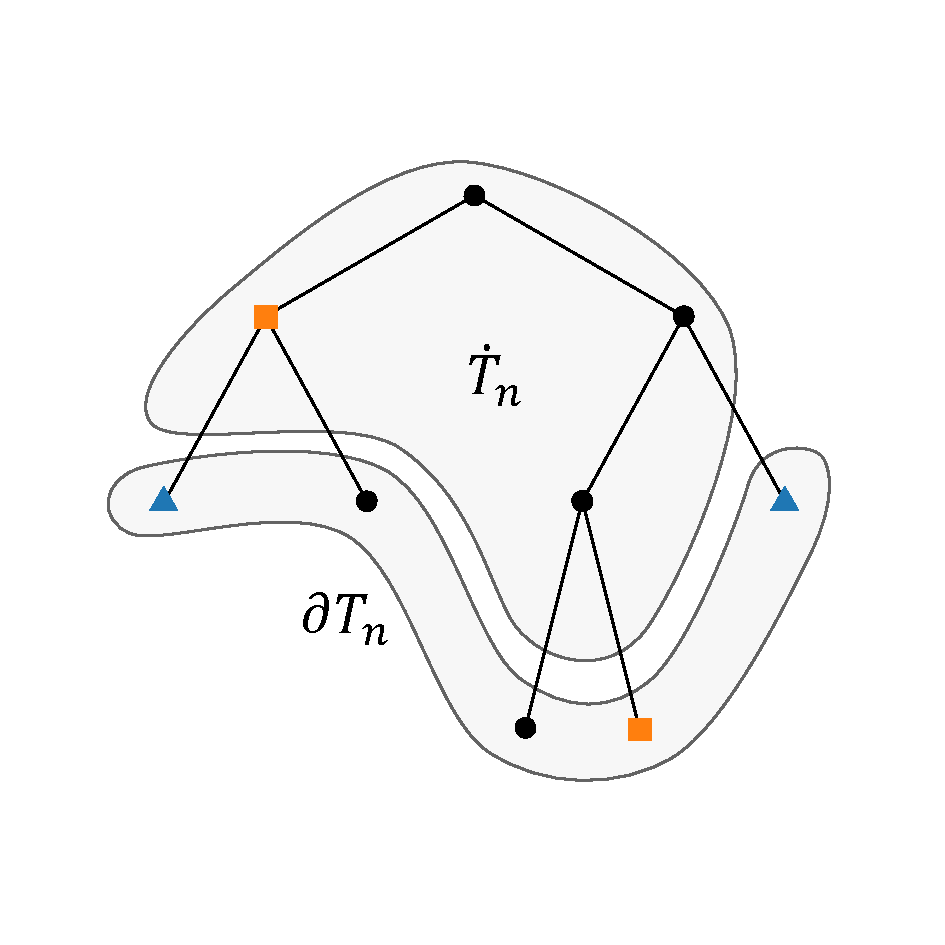
\includegraphics[trim={1.8cm 2.2cm 1.9cm 2.7cm}, clip,width=0.46\linewidth]{img/tree_1}
	\hfill
	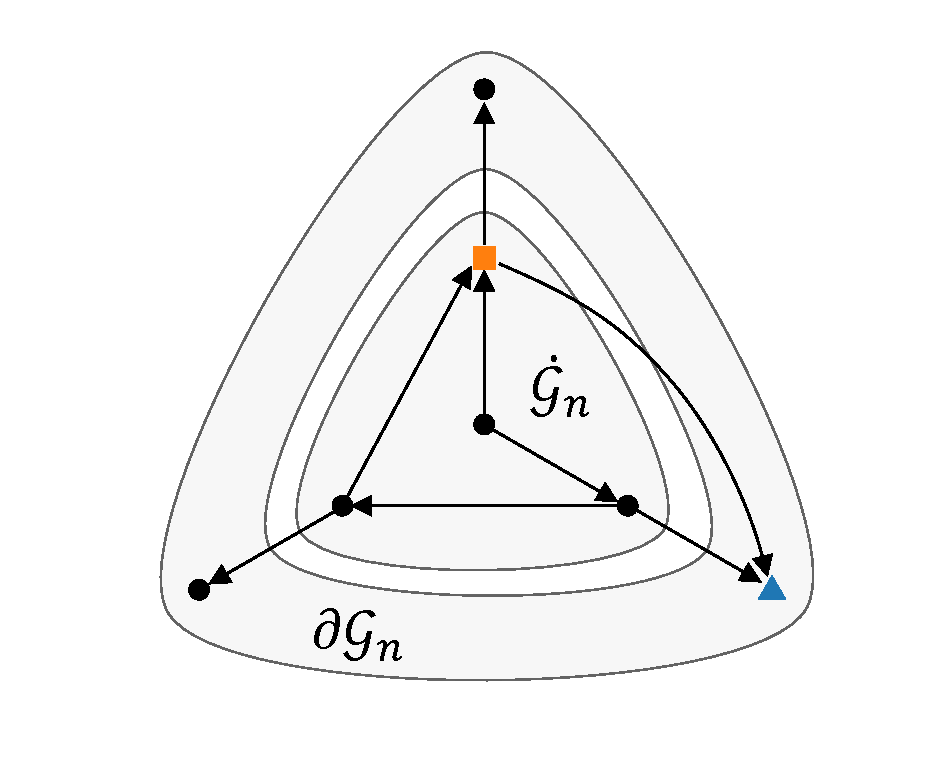
\includegraphics[trim={1.8cm 1.2cm 1.9cm 0.8cm}, clip,width=0.46\linewidth]{img/graph_1}
	\caption{Illustration of the tree $\Tau_n$ (left) and the graph $\cG_n$ (right) built from the same observed transitions. The root of the tree corresponds to the central graph node. In the tree, two nodes with the same colour and shape (not black round) lead to the same state.}
	\label{fig:structures}
\end{figure}

In a tree, a node of depth $h$ represents a sequence of actions $a\in A^h$. The \textit{root} of the tree corresponds to the empty action sequence, and hence to the initial state $s_0\in S$. At iteration $n$, we denote the current tree as $\Tau_n$. Borrowing notations from topology, we denote its set of internal nodes as $\inte{\Tau}_n$ and its set of external nodes (the leaves) as $\ext{\Tau}_n$. Note that since the MDP is deterministic, a sequence of action $a$ is associated with its final state denoted $s(a)$, but this association is not one-to-one: several sequences of action can lead to the same state, which will be represented several times in the tree.

In a graph, the nodes represent states $s\in S$, and the edges represent transitions between states. The \textit{source} of the graph corresponds to the initial state $s_0$. At iteration $n$, we denote the current graph as $\cG_n$, its set of internal nodes as $\inte{\cG}_n$ and its set of \textit{sinks} as $\ext{\cG}_n$.

Both structures are built iteratively from a single starting node, by selecting an external node (leaf or sink) to expand. The \emph{expansion} of a node $a$ or $s$ refers to calling the generative model to sample the reward $r$ and next state $s'$ for each action $a\in A$, and adding child nodes to the data structure. In a tree, the expansion of a node $a\in A^h$ always lead to the creation of new leaves that represent the suffix sequence of action $ab\in A^{h+1},\, b\in A$. The maximum depth of an expanded node in $T_n$ is denoted $d_n$. In contrast, in a graph the next state $s'$ reached from $s,a$ might already be present in $\cG_n$, in which case we add the edge between $s$ and $s'$ without creating a new node.
These data structures can be used to store information about the MDP, such as the transitions and rewards $r(s, a)$, or other informations useful for planning.


\subsection{Optimistic planning}

A planning algorithm is typically composed of two main rules:
%\begin{enumerate*}[label=(\roman*)]
	(i) A \emph{sampling rule}, that selects promising transitions to simulate at each iteration $n$; 
	(ii) A \emph{recommendation rule}, that recommends a good first action $a_n$ to take (in $s_0$).
%\end{enumerate*}
%The pseudo-code of generic planning algorithm is provided in \Cref{alg:generic}.
%\begin{algorithm}
%	\caption{A generic planning algorithm}
%	\label{alg:generic}
%	\DontPrintSemicolon
%	\For{each iteration $n$}{
%		Select the node $b_n$ (or $\hat{s_n}$) to expand according to the \textbf{sampling rule}.\;
%		\For(\Comment*[f]{Node expansion}){action $a\in A$}{
%			Simulate the transition $r, s' \sim P\left(r, s' \condbar s, a\right)$ from the generative model.\;
%			Insert the observed transition to the data structure accordingly.
%		}
%	}
%	\Return the recommended action $a_{n}$ according to the \textbf{recommendation rule}.\;
%\end{algorithm}
These rules can be chosen with the goal of minimising the simple regret $r_n$.
A popular approach is to follow the principle of \emph{Optimism in the Face of Uncertainty} (OFU) \citep[see][]{Munos14}, which consists in exploring the option that maximises an upper-bound of the true objective. In the context of planning, it has been applied by forming bounds on the value function $V$.

\begin{definition}[Value bounds]
\textbf{On trees.} We denote by $L:\Tau_n \rightarrow \Real$ and  $U:\Tau_n \rightarrow \Real$ a lower-bound and upper-bound for the state value $V$ defined on the tree $\Tau_n$, such that
\begin{equation*}
    \forall a\in\Tau_n, \qquad L(a) \leq V(s(a)) \leq U(a).
\end{equation*}

\textbf{On graphs.} Likewise, we denote by $\cL:\cG_n \rightarrow \Real$ and  $\cU:\cG_n \rightarrow \Real$ a lower-bound and upper-bound for the state value $V$ defined on the graph $\cG_n$, such that
\begin{equation*}
\forall s\in\cG_n, \qquad \cL(s) \leq V(s) \leq \cU(s).
\end{equation*}
\end{definition}

Following the OFU principle, at iteration $n$ we must leverage available information to design an upper-bound $U_n$ (or $\cU_n$) on $V$ as tight as possible. Then, in order to select a promising external node to expand, the sampling rule starts from the root (or source) and follows the optimistic strategy of always selecting the action which maximises $U_n$ (or $\cU_n$), until reaching an optimistic leaf (or sink) to expand. This strategy was used with great success in \citep[e.g.][]{Kocsis06UCT, Hren2008optimistic, Bubeck2010open, Busoniu2012optimistic}.

For instance, since we assume that the rewards are bounded in [0, 1], trivial bounds on $V(s)$ are
$0 \leq V(s) \leq V_{\max} \eqdef \sum_t \gamma^t 1 = {1}/({1-\gamma})$. But these trivial bounds are the same for every node, which makes them non-informative, and do not make use of the observed information. However, they can be used as a valid starting point. Each observed transition can then be used to tightened these bounds, by resorting to the Bellman optimality operator.

\begin{definition}[Bellman optimality operator]
	\label{def:bellman}
	\textbf{On trees.} We define the Bellman optimality operator $B_n$ on the tree $\Tau_n$ as:
	\begin{equation}
	\label{eq:bellman-tree}
	B_n(f)(a) \eqdef \begin{cases}
	\max_{b\in A} r(s(a), b) + \gamma f({ab})
	& \text{if $a\in\inte{\Tau}_n$;} \\
	f(a) & \text{if $a\in\ext{\Tau}_n$;}
	\end{cases}
	\end{equation}
	where $f:\Tau_n \rightarrow \Real$ is a real-valued function of tree nodes, such as the value bounds $L,U$.
	 
	\textbf{On graphs.} Likewise, we define the Bellman optimality operator $\cB_n$ on the graph $\cG_n$:
	\begin{equation}
	\label{eq:bellman-graph}
	\cB_n(f)(s) \eqdef \begin{cases}
	\max_{b\in A} r(s, b) + \gamma f(P(s,b))
	& \text{if $s\in\inte{\cG}_n$;} \\
	f(s) & \text{if $s\in\ext{\cG}_n$.}
	\end{cases}
	\end{equation}
	The updates with both Bellman operators are depicted in \Cref{fig:bellman}.
\end{definition}

%\begin{remark}
%	For ease of notation, we will sometimes drop the $n$ index on $B$ and $\cB$ when it is non-ambiguous.
%\end{remark}


\begin{figure}[tp]
	\centering
	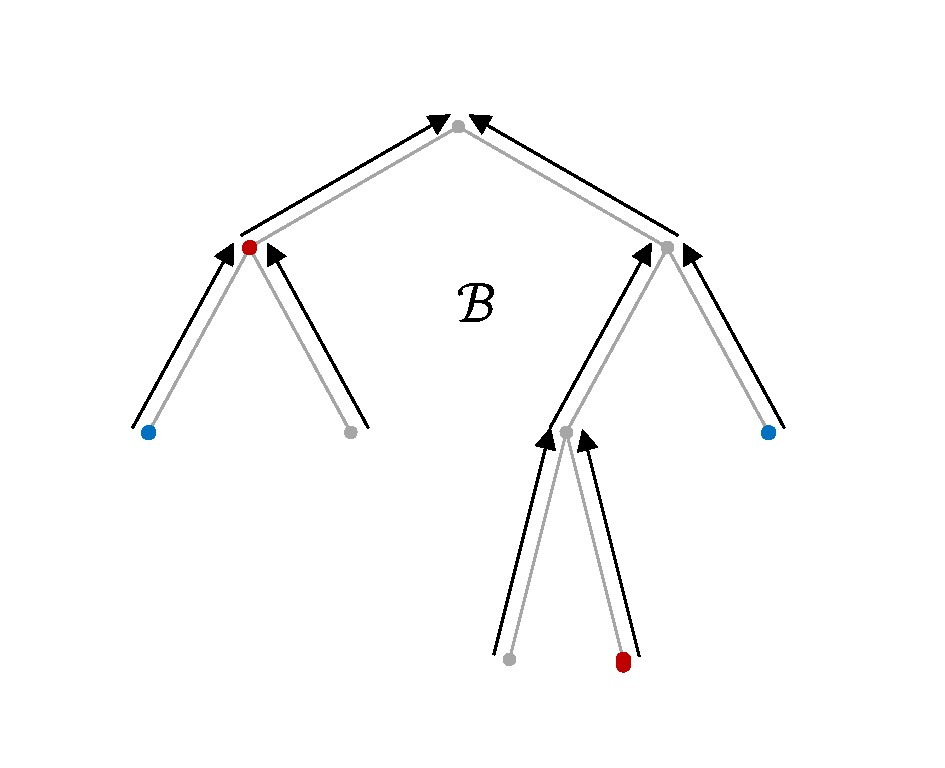
\includegraphics[trim={2.0cm 2.9cm 2.5cm 3.1cm}, clip,width=0.44\linewidth]{img/tree_2}
	\hfill
	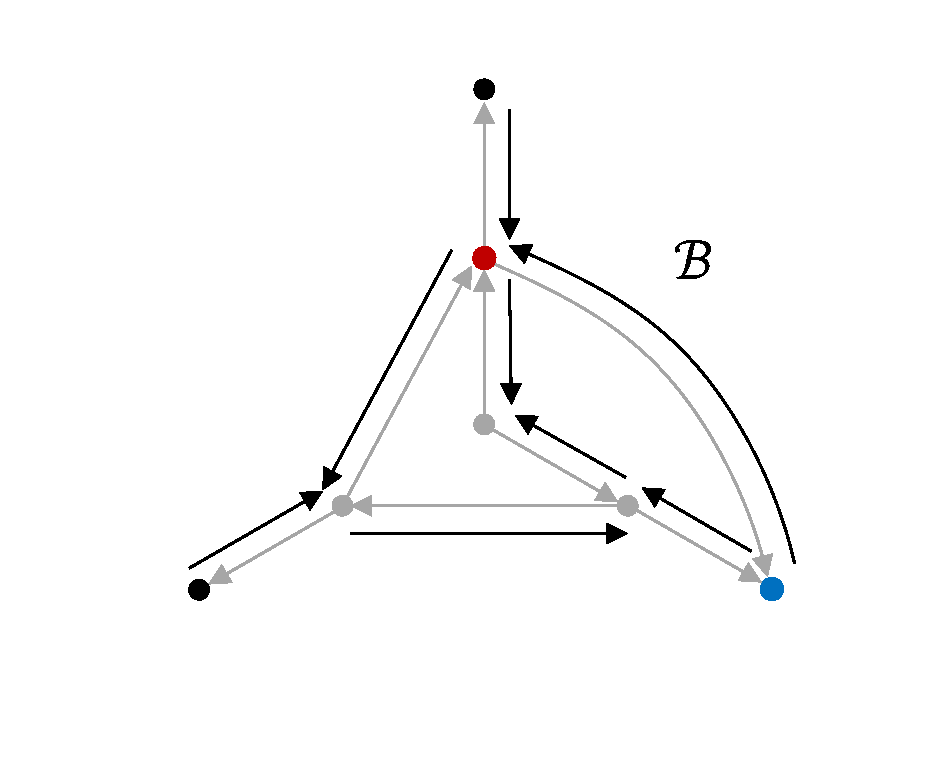
\includegraphics[trim={2.7cm 2.7cm 2.7cm 1.1cm}, clip,width=0.44\linewidth]{img/graph_2}
	\caption{Illustration of the Bellman backup operators $B$ (left) and $\cB$ (right). Notice that $B_n$ only propagates information upward in the tree.}
	\label{fig:bellman}
\end{figure}

\citet{Hren2008optimistic} used this Bellman operator $B_n$ in their \texttt{OPD} algorithm to define a pair of bounds $(L_n,\, U_n)$ at each iteration $n$. They use trivial bounds at the leaves, and backup these estimates up to the root by iteratively applying $B_n$. We can show that, under a \textit{monotonicity} condition (satisfied by the trivial bounds $0$ and $V_{max}$), applying $B_n$ can only tighten a bound and converges in a finite time.

\begin{definition}[Monotonicity]
	A pair of bounds ($L$, $U$) or $(\cL, \cU)$ is \emph{monotonic} if they are respectively non-decreasing and non-increasing along transitions:
	\begin{align*}
	\forall a\in{\Tau}_n, \quad & L(a) \leq B_n(L)(a), & U(a) & \geq B_n(U)(a)\\
	\forall (s)\in\inte{\cG}_n, \quad &\; \cL(s) \leq \cB_n(\cL)(s),&   \cU(s) & \geq \cB_n(\cU)(s)
	\end{align*}
\end{definition}

\begin{lemma}[Properties of $B_n$]
	\label{lem:properties-b-tree}
	\begin{enumerate}[(i)]
		\item $B_n$ preserves monotonicity and tightens monotonic bounds: $$
		\text{if } L\leq V\leq U \text{, then } L \leq B_n(L) \leq V \leq B_n(U) \leq U;
		$$
		\item The sequence $B_n^k = \underbrace{B_n \circ \dots\circ B_n}_{\text{$k$ times}} $ converges in a finite time $k=d_n$, where $d_n$ is the depth of $T_n$. 
	\end{enumerate}
\end{lemma}
This enables \citet{Hren2008optimistic} to define\footnote{We use an iteration of operators while a recursive definition was used originally.} non-trivial valid bounds on $V$:
\begin{align}
\label{eq:opd-bounds}
L_n \eqdef B_n^{d_n}(0), \qquad U_n \eqdef B_n^{d_n}(V_{\max}),
\end{align}
where $0$ is the null function. The corresponding \texttt{OPD} algorithm is described in \Cref{alg:opd}.

\begin{algorithm}[ht]
	\caption{The \emph{Optimistic Planning of Deterministic Systems} (\OPD) algorithm from \citep{Hren2008optimistic}.}
	\label{alg:opd}
	\DontPrintSemicolon
	\For{each iteration $n$}{
		Compute the bounds $L_n = B_n^{d_n}(0)$ and $U_n = B_n^{d_n}(V_{\max})$.\; 
		
		$b_n\gets \emptyset$\;
		
		\While{the node $b_n\in\inte{\Tau}_n$ is internal}{
			$b_n\gets \displaystyle\argmax_{a'\in b_n A} r(a') + \gamma U_n(a')$ \Comment*[r]{Optimistic sampling rule}
		}
		\For(\Comment*[f]{Node expansion}){action $a\in A$}{
			Simulate $r \gets r(s(b_n),a)$ and $s' \gets P(s(b_n),a)$.\;
			
			Add a new leaf $b_n a$ to $\Tau_{n+1}$, with associated reward $r$.\;
		}
	}
	\Return $\displaystyle\argmax_{a\in A} r(s, a) + \gamma L_n(a)$. \Comment*[r]{Conservative recommendation rule}\;
\end{algorithm}

Likewise, we show that the graph version $\cB_n$ verifies similar properties.
\begin{lemma}[Properties of $\cB_n$]
	\label{lem:properties-b-graph}
	\begin{enumerate}[(i)]
		\item $\cB_n$ preserves monotonicity and tightens monotonic bounds: $$
		\text{if } \cL\leq V\leq \cU \text{, then } \cL \leq \cB_n(\cL) \leq V \leq \cB_n(\cU) \leq \cU;
		$$
		\item $\cB$ is a $\gamma$-contraction, and we denote $\cB_n^{\infty} \eqdef \lim_{k\rightarrow \infty} \cB_n^k$.
	\end{enumerate}
\end{lemma}
This motivates us to propose \Cref{alg:gbop-d}, following the approach of \Cref{alg:opd} adapted to a graph structure.

\begin{algorithm}[ht]
	\caption{Our proposed \emph{Graph-Based Optimistic Planning for Deterministic systems} (\GBOPD) algorithm.}
	\label{alg:gbop-d}
	\DontPrintSemicolon
	\For{each iteration $n$}{
		\nl Compute the bounds $\cL_n = \cB_n^{\infty}(0)$ and $\cU_n = \cB_n^\infty(V_{\max})$.\; 
		
		$s_n \gets s_0$\;
		
		\While{the node $s_n\in\inte{\cG}_n$ is internal}{
			\nl $s_n\gets \displaystyle\argmax_{s'} r(s_n, a) + \gamma \cU_n(s')$ \Comment*[r]{Optimistic sampling rule}
		}
		\For(\Comment*[f]{Node expansion}){action $a\in A$}{
			Simulate $r \gets r(s_n, a)$ and $s' \gets P(s_n,a)$.\;
			
			Get or create the node $s'$ in $\cG_{n+1}$, and add the transition $(s_n,a) \rightarrow s', r$.\;
		}
	}
	\Return $\displaystyle\argmax_{a\in A} r(s,a) + \gamma \cL_n(s(a))$. \Comment*[r]{Conservative recommendation rule}
\end{algorithm}

\begin{remark}[Termination and complexity]
One key difficulty both in the design and analysis of the algorithm is the correct handling of loops in the graph.
Indeed, there are two procedures in \GBOPD that may not terminate in finite time whenever $\cG_n$ contains a loop:
%\begin{enumertate*}[label=(\roman*)]
	 the computation of $\cB_n^\infty$ (line 1) and 
	 the sampling rule loop (line 2).
%\end{enumerate*}
We handle these steps carefully in the Supplementary Material, where we discuss an approximate implementation in which these two procedures are stopped whenever they reach a desired accuracy $\varepsilon$, along with an analysis of the corresponding time complexity and impact on the performance.
\end{remark}

Though both algorithms share a similar design, we claim that using graphs provides substantial theoretical and practical performance improvements, and back up this statement in \Cref{sec:analysis,sec:experiments}.

\section{Analysis}
\label{sec:analysis}

Comparing \OPD and \GBOPD directly is difficult since they do not involve the same structure, which implies implicit differences in their behaviours. Studying them under a common framework makes these differences explicit. To leverage the analysis of \OPD by \citet{Hren2008optimistic}, we will frame \GBOPD as a tree-based planning algorithm: the graph operator $\cB$ will be represented as tree backup $B$ applied on an \emph{unrolled} tree $T(\cG_n)$, defined below.

\subsection{Background on the sample complexity of \OPD}

First, we recall the analysis of \citet{Hren2008optimistic} and introduce some notations.

\begin{definition}[Sequence values]
The value of a finite \textbf{sequence} of actions $a\in A^h$ is:
\begin{equation*}
\label{eq:state_value}
    V(a) = R(s_0,a) + \gamma^{h} V(s(a)),
\end{equation*}
where $R(s, a) = \sum_{t=0}^{h-1} \gamma^t r_t$ is the return obtained by executing the sequence of actions $a$ starting from the state $s$. We also denote $V^\star = \max_{a\in A}V(a)$ the value of the best action.
\end{definition}

This enables to define a measure of the difficulty of a planning problem.

\begin{definition}[Difficulty measure]
We define the near-optimal branching factor $\hlrb{\kappa}$ of an MDP as
\begin{equation}
\hlrb{\kappa = \limsup_{h\rightarrow\infty} |\hlrb{\Tau_h^\infty}|^{1/h}} \in [1, K]
\end{equation}
where $\Tau^\infty_h = \displaystyle \left\{a\in A^h: V^\star-V(a) \leq \frac{\gamma^h}{1-\gamma}\right\}$ is the set of near-optimal nodes at depth $h$.
\end{definition}

This problem-dependent measure $\hlrb{\kappa}$ is the branching factor of the subtree $T^\infty=\bigcup_h T_h^\infty$ of near-optimal nodes that can be sampled by \OPD, and acts as an effective branching factor as opposed to the true branching factor $K$. When $\hlrb{\kappa}$ is small, fewer nodes must be explored at a given depth allowing the algorithm to plan deeper for a given budget $n$. Thus, it directly impacts the simple regret that can be achieved by \OPD when run on a given MDP.


\begin{theorem}[Regret bound of \citealt{Hren2008optimistic}]
\label{thm:regret-opd}
The \Cref{alg:opd} enjoys the following regret bound:
\begin{align*}
\quad r_n = \tilde{\cO}\left( n^{-\log \frac{1}{\gamma}/\hlrb{\log\kappa}}\right),
\end{align*}
where $f_n = \tilde{\cO}(n^{-\alpha})$ means that for any $\alpha'<\alpha$, $f_n = \cO(n^{-\alpha'})$, for all $\alpha\in \Real_+ \cup \{+\infty\}$.

\end{theorem}

The near-optimal branching factor $\hlrb{\kappa}$ is related \citep{Bubeck2010open} to the near-optimality dimension studied in the online optimisation literature \citep[see e.g.][]{Bubeck2009,Munos2011}.
It is typically small in problems where there is one single optimal trajectory, of which any deviation can be quickly dismissed as suboptimal. Conversely, $\kappa$ is large when many sub-optimal trajectories cannot be distinguished easily based on their values, which requires the exploration of a large part of the tree $T$ of branching factor $K$. 


\subsection{Motivation for an improved regret bound}

We start by reformulating the sampling rule used for the \texttt{OPD} algorithm. To that end, notice that when some bounds $(L,\,U)$ on the state values $V(s(a))$ are available, they also induce bounds $(\overline{L},\, \overline{U})$ on values $V(a)$ of sequences of actions $a$ of length $h$ defined as:
\begin{equation*}
%\label{eq:sequence_value}
\underbrace{R(s_0,a) + \gamma^{h} L(a)}_{\overline{L}(a)} \leq V(a) \leq \underbrace{R(s_0,a) + \gamma^{h} U(a)}_{\overline{U}(a)}.
\end{equation*}

One can easily see that, since the $(L_n,\,U_n)$ used in the optimistic sampling rule described in \Cref{alg:opd} are invariant by $B_n$ by definition, this rule can be equivalently expressed as:
\begin{equation}
\label{eq:sampling_rule}
b_n \in \argmax_{a\in\ext{\Tau}_n} \overline{U}_n(a).
\end{equation}
Likewise, the conservative recommendation rule returns the first action of:
\begin{equation}
\label{eq:recommendation_rule}
a_n \in \argmax_{a\in\ext{\Tau}_n} \overline{L}_n(a)
\end{equation}


As shown in \Cref{fig:bellman}, in a tree the Bellman operator $B_n$ only propagates the information upward, and the leaves cannot be updated. Thus, $U_n = B_n^{d_n}(V_{\max})$ and $V_{\max}$ coincide on $\ext{\Tau}_n$ which means that the sampling rule of \texttt{OPD} can be summarized as using \eqref{eq:sampling_rule} with the trivial upper-bound $U_n = V_{\max}$.
Likewise, the recommendation rule simply uses \eqref{eq:recommendation_rule} with the trivial lower-bound $L_n = 0$. Thus, \texttt{OPD} amounts to simply using the trivial bound $(0,\, V_{\max})$ on leaf nodes, and does not make use of all the available information in $\Tau_n$ to improve these bounds.

Let us now assume for the moment that we have access to tighter bounds $(L,\,U)$ provided by an oracle: $$0\leq L\leq V\leq U\leq V_{\max}.$$
\vspace*{-0.5cm}
\begin{definition}[A finer difficulty measure]
We define the near-optimal branching factor \emph{according to the bounds $(L,\,U)$} as 
\begin{equation}
\hlbb{\kappa(L,U) \eqdef \limsup_{h\rightarrow\infty} \left|\Tau_h^\infty(L,U)\right|^{1/h}}\in[1, K], 
\end{equation}
where
$ \displaystyle
     {\Tau_h^\infty(L,U)}=\left\{a\in A^h: V^\star - V(a)\leq \gamma^{h}(U(a)-L(a))\right\}.
$
\end{definition}

\begin{lemma}
\label{lem:shrink}
This branching factor shrinks as the bounds $(L,\,U)$ get tighter:
\[L_2\leq L_1\leq V\leq U_1\leq U_2\implies \kappa(L_1,U_1) \leq \kappa(L_2,U_2).\]
In particular, $\hlbb{\kappa(L,U)} \leq \hlrb{\kappa}$.
\end{lemma}

\begin{theorem}
\label{thm:regret-bound-U}
Let $L \leq V\leq U$ monotonic bounds, then planning with $L$ and $U$ in \eqref{eq:sampling_rule} and \eqref{eq:recommendation_rule} yields the following simple regret bound:
\begin{equation*}
r_n = \tilde{\cO}\left(n^{-\log \frac{1}{\gamma}/\hlbb{\log \kappa(L,U)}}\right).
\end{equation*}
\end{theorem}


This theorem states that we can potentially improve the performance of the planning algorithm if we manage to find bounds $(L,\, U)$ that are tighter than the trivial ones at the leaves $\ext{\Tau_n}$, which may be possible if we have already seen the states corresponding to this leaves, but it does not explain how to obtain such bounds. In the next subsection, we describe a method to build a sequence of increasingly tight bounds $(L_n,\, U_n)$, at each planning iteration $n$. The corresponding regret bound, our main result, is stated in \Cref{thm:regret-gbop}.


\subsection{Unrolling the tree to tighten the bounds}
\label{sec:unrolling}

In order to reproduce the behaviour of \Cref{alg:gbop-d} on a tree structure, we rely on the following observation:  expanding a node $s$ in $\cG_n$ simultaneously expands all the paths leading to this node.
To account for this observation in the analysis, we will consider an \emph{unrolling} operator $T$, illustrated in \Cref{fig:unroll}, that builds a potentially infinite tree $T(\cG_n)$ containing every sequence of action that can be traversed in a graph $\cG_n$.

\begin{equation}
T(\cG_n) = \{a\in A^h: s_{t+1} \in \cG_n \text{ with } s_{t+1} = P(s_{t}, a_t)\text{ for } 0 \leq t < h\}
\end{equation}

\begin{figure}[htp]
	\centering
	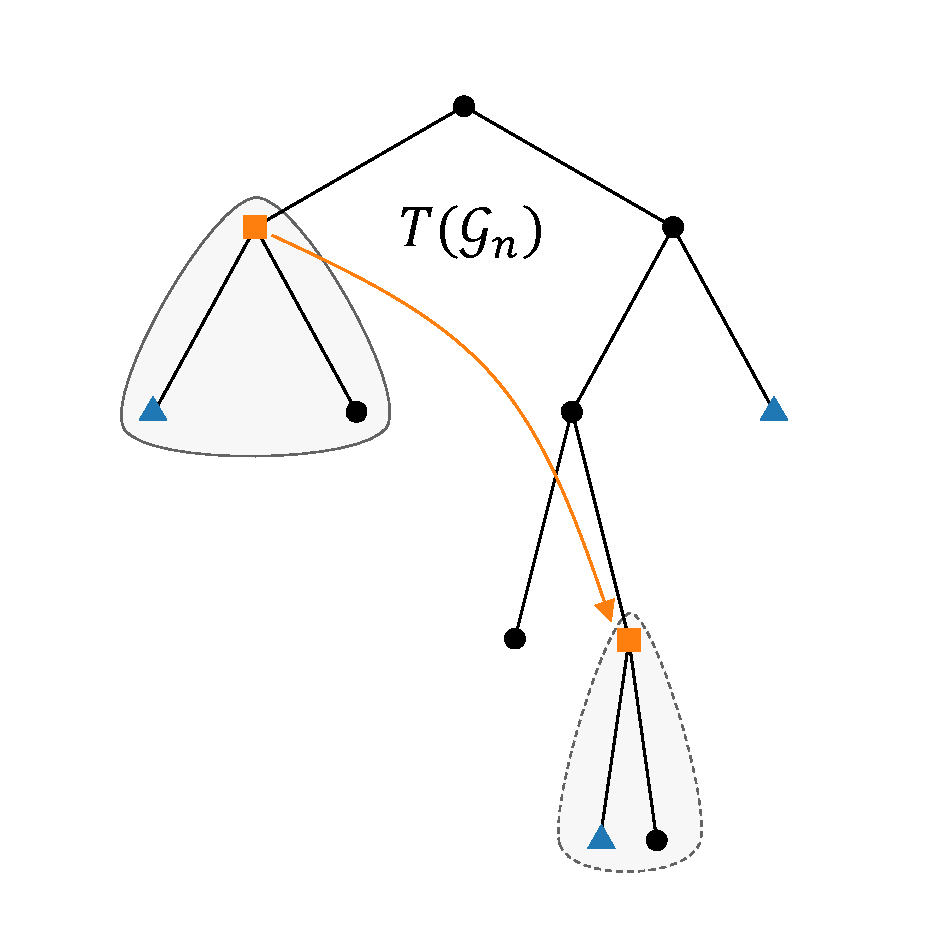
\includegraphics[trim={2.cm 1cm 2.5cm 1cm}, clip, width=0.44\textwidth]{img/tree_5.pdf}
	\caption{The tree $T(\cG_n)$ obtained by unrolling $\cG_n$. Contrary to $T_n$ shown in \Cref{fig:structures}, the orange leaf $a$ is expanded at the same time as the internal orange node, which enables to tighten its value bounds $(L_n(a), U_n(a))$ by applying $B_n$.}
	\label{fig:unroll}
\end{figure}
We analyse \GBOPD though the prism of $T(\cG_n)$, which is only used as a theoretical tool. 

We can define the counterpart of the bounds $(\cL_n, \cU_n)$ in the same way as \eqref{eq:opd-bounds} applied to $T(\cG_n)$ rather than $T_n$, except that the depth $d_n$ of $T(\cG_n)$ can now be infinite:
\begin{align}
\label{eq:gbop-t-bounds}
L_n = B_n^{\infty}(0), \qquad U_n = B_n^{\infty}(V_{\max}).
\end{align}
This definition is equivalent to that of \GBOPD in the sense that:
\begin{lemma}[Bound equivalence]
	\label{lem:equivalence}
For any sequence of action $a\in T(\cG_n)$, we have $L_n(a) = \cL_n(s(a))$ and $U_n(a) = \cU_n(s(a))$.	
\end{lemma}

In $T(\cG_n)$, the unrolling mechanics behave as if any leaf $a$ sharing the same state $s(a)$ as an internal node $a'$ was automatically expanded, and thus had its bound $L_n(a), U_n(a)$ tightened by the Bellman backup $B_n$ to a sub-interval of the trivial bounds $(0, V_{\max})$ that are used in \OPD.

The sampling and recommendation rules of \GBOPD amount to running those of \OPD on the tree $T(\cG_n)$, except that the sampled sequence $b_n$ and recommended sequence $a_n$ can now have infinite depth since $T(\cG_n)$ itself can be infinite (we say that $a_n$ and $b_n$ are represented by nodes of infinite depth). In the sequel, we analyse how these rules behave on $T(\cG_n)$.

\begin{lemma}[Expansion]
	\label{lem:expansion-bound}
	Any node $a$ of depth $h$ traversed by the optimistic sampling rule of \GBOPD at iteration $n$ belongs to $T_h^\infty(L_n, U_n)$: 
	\begin{equation}
	\label{eq:expansion-regret}
	V^\star-V(a) \leq \gamma^h(U_n(a)-L_n(a)).
	\end{equation}
	
	In particular, if the sampling rule samples an infinite sequence $a\in A^\infty$, it is an optimal sequence, and we write that \eqref{alg:gbop-d} also holds for $a$ with $h=\infty$.
\end{lemma}


\begin{lemma}[Recommendation]
	\label{lem:recommendation-bound}
	The action $a_n$ recommended by \GBOPD has a simple regret $r_n \leq \frac{\gamma^{d_n}}{1-\gamma}$, where $d_n\in\Real\cup\{\infty\}$ is the maximal depth of expanded nodes in $T(\cG_n)$.
\end{lemma}
Note that even though $T(\cG_n)$ can be infinite, there is only one node $b_t$ that is selected for expansion at each iteration $t\leq n$.

\subsection{Regret guarantee}

In \Cref{thm:regret-bound-U}, we assumed that some bounds $(L,\,U)$ were revealed by an oracle and available from the onset for planning. In \eqref{eq:gbop-t-bounds}, we instead built a \emph{sequence} of bounds $(L_n,U_n)_{n\geq 0}$ \eqref{eq:gbop-t-bounds} that is non-increasing in the sense of inclusion, i.e. $0\leq \dots\leq L_{n-1}\leq L_n\leq V\leq U_n\leq U_{n-1}\leq \dots\leq V_{\max}$.

We can consider the sequence $\kappa_n = \kappa(L_n, U_n)$. By Lemma \ref{lem:shrink}, it is non-increasing and lower-bounded by $1$, thus converges. Let $\hlgb{\kappa_\infty = \lim_{n\rightarrow\infty} \kappa(L_n, U_n)} \in[1,K]$.

\begin{theorem}
\label{thm:regret-gbop}
\GBOPD enjoys the following regret bound, with $\hlgb{\kappa_\infty} \leq \hlrb{\kappa}$: 
\begin{align*}
r_n = \tilde{\cO}\left(n^{-\log \frac{1}{\gamma}/\hlgb{\log \kappa_\infty}}\right).
\end{align*}
\end{theorem}

Intuitively, $\kappa_\infty$ should be much lower than $\kappa$ in problems where trajectories overlap a lot. For instance, it will be the case when two actions cancel each-other out (e.g. moving left or right), or are commutative (e.g. placing pawns on a board game). However, this is merely an intuition. We now show that there exist problem instances in which $\hlgb{\kappa_\infty} < \hlrb{\kappa}$, which is a legitimate concern since their non-existence would make \Cref{thm:regret-gbop} trivial.

\subsection{Illustrative example}

In Proposition \ref{prop:illustrative-example}, we consider a toy MDP $\cM$ shown in \Cref{fig:mdp}. The transitions are described visually while the rewards are defined as follows: let $0\leq r^\star\leq \gamma$, and $ r^- = r^\star - \frac{\gamma}{1-\gamma} S$, $r^+ = r^\star + S$ with $S = r^\star\left(\frac{1}{\gamma} - 1\right).$ Note that this choice ensures that $r^\star, r^-, r^+$ and $S$ are all in $[0, 1]$.

\begin{figure}[htp]
    \centering
    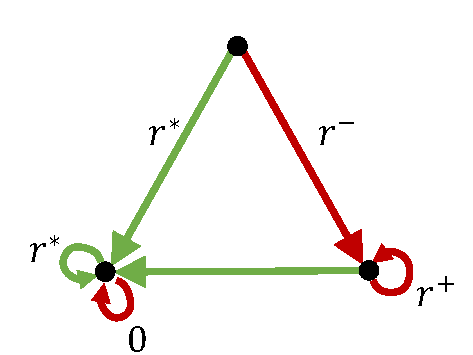
\includegraphics[trim={0.5cm 0.0cm 0.3cm 0.6cm}, clip, width=0.35\textwidth]{img/mdp.pdf}
    \caption{A toy MDP with three states and $K \geq 2$ actions. We start in the top state. The first action $a_1$ is represented by \textcolor{Green}{green} arrows, and all other actions $a_2, \dots, a_K$ are represented by \textcolor{Orange}{orange} arrows. The rewards are shown next to the transitions.}
    \label{fig:mdp}
\end{figure}

\begin{proposition}[Branching factors]
\label{prop:illustrative-example}
The MDP $\cM$ verifies $\hlrb{\kappa = K-1}$ and $\hlgb{\kappa_\infty = 1}$.
% :
% \begin{enumerate}[label=(\roman*)]
%     \item $\hlrb{\kappa = K-1}$;
%     \item $\hlgb{\kappa_\infty = 1}$.
% \end{enumerate}
\end{proposition}
This result confirms that \Cref{thm:regret-gbop} is non-trivial since we exhibit a problem for which $\hlgb{\kappa_\infty} < \hlrb{\kappa}$ (when $K\geq 3$), and legitimates our attempt to improve planning performances by merging the tree into a graph.


\section{Extension to Stochastic Systems}
\label{sec:stochastic}

The approach developed in \Cref{sec:gbopd,sec:analysis} consists in using state similarity to tighten a pair of lower and upper bounds $(L,\,U)$ for the value function $V$. Thus, any planning algorithm that is based on such bounds can benefit from this insight, and any theoretical result based on the validity and rate of convergence of these bounds will be preserved.  

\paragraph{Confidence intervals for rewards.}

When the reward distribution $P\left(r \condbar s,a\right)$ is stochastic, deviation inequalities can be used to design a confidence interval $[\ell_t(s,a), u_t(s,a)]$ over its expected value $\expectedvalue\left[r | s,a\right]$. For instance, the Chernoff-Hoeffding deviation inequality was used to design confidence intervals in \citep{Kocsis06UCT,Bubeck2010open,Kaufmann2017}.
In recent works \citep{Leurent2019practical, Jonsson2020planning}, the tighter Kullback-Leibler confidence interval is preferred:
\begin{align*}
u_t(s,a) &\eqdef \max \left\{v : \kl\!\big(\hat{r}_t(s,a),v\big) \leq \frac {\beta^r(n_t(s,a), n)} {n_t(s,a)} \right\},\\
\ell_t(s,a) &\eqdef\min \left\{v : \kl\!\big(\hat{r}_t(s,a),v\big) \leq \frac {\beta^r(n_t(s,a), n)} {n_t(s,a)} \right\},
\end{align*}
where $n_t(s,a)$ is the number of times the transition $(s,a)$ was visited, $\hat{r}_t(s,a)$ is the empirical mean reward, $\beta^r$ is an exploration function and $\kl(u,v)$ is the binary Kullback-Leibler divergence between Bernoulli distributions: $\kl(u,v) = u \log \tfrac {u} {v} + (1-u) \log \tfrac {1-u} {1-v}$.

\paragraph{Confidence region for transitions.}

Likewise, when the transition distribution $P\left(s' | s,a\right)$ is stochastic, a confidence set on the probability vector $p(\cdot|s,a)$ can be defined as
$\cC_t(s,a) \eqdef \left\{p\in \Sigma_S :  \KL\!\big(\hp_t(\cdot|s,a),p\big) \leq \frac {\beta^p(n_t(s,a), n)} {n_t(s,a)}\right\}$,
where $\hp_t(\cdot|s,a) \eqdef n_t(s,a,\cdot) / n_t(s,a)$ is the empirical distribution, $\Sigma_S$ is the probability simplex over $S$, $\beta^p$ is an exploration function and $\KL(p,q)= \sum_{s \in S}  p(s) \log \tfrac{ p(s)} {{q}(s)}$ is the Kullback-Leibler divergence between categorical distributions.

\paragraph{Bellman operator with stochasticity.}

In this work, we do not discuss the tuning of $\beta^r$, $\beta^p$, but simply assume that they are chosen such that the rewards and transitions belong to their confidence regions with sufficiently high probability to obtain performance guarantees for the planning algorithm. For more details on such a choice, refer to \citep[e.g.][]{Leurent2019practical, Jonsson2020planning}. We modify the Definition \ref{def:bellman} of $\cB_t$ as:

\begin{align*}
\cB_t^+(\cU)(s) &= \max_{a\in A} \left[u_t(s,a) + \gamma \max_{q \in \cC_t(s,a)} \sum_{s'} q(s'|s,a) \cU(s')\right], \\
\cB_t^-(\cL)(s) &= \max_{a\in A} \left[\ell_t(s,a) + \gamma \min_{q \in \cC_t(s,a)} \sum_{s'} q(s'|s,a)\cL(s')\right],
\end{align*}
for all $s\in\inte{\cG_n}$, where the maximum and minimum over these Kullback-Leibler confidence regions $\cC_t(s,a)$ can be computed as explained in \citep[Appendix A of][]{Filippi2010optimism}. Under the event that every confidence regions $[\ell_t(s,a), u_t(s,a)]$ and $\cC_t(s,a)$ are valid at time $t$, the Lemma \ref{lem:properties-b-graph} still holds for $\cB_t^-, \cB_t^+$.

\paragraph{Structure of the planning algorithm}

In the deterministic setting, once a transition has been observed, it is known with certainty and doesn't need to be sampled ever again, which is why only external nodes $\ext{\cG_n}$ are sampled in \GBOPD. Conversely, in the stochastic setting the expected reward and transition probabilities must be estimated from samples, which implies that internal nodes $\inte{\cG_n}$ must be sampled as well. Then, it is common to adopt and episodic setting where we sample trajectories of a fixed horizon $H$, tuned depending on the budget $n$. This is the case in  \citep[e.g.][]{Kearns02SS,Kocsis06UCT,Bubeck2010open,Feldman14BRUE,Leurent2019practical,Jonsson2020planning}. We also follow this scheme in our proposed \GBOP

\begin{algorithm}[ht]
	\caption{\emph{Graph-Based Optimistic Planning} (\GBOP) algorithm.}
	\label{alg:gbop}
	\DontPrintSemicolon
	\For{trajectory $m$ in $[1, M]$}{
		\For{time $t$ in $[1, H]$}{
			$n \gets (m - 1)H + t$.\;
			Compute the bounds $\cL_n = (\cB_n^-)^{\infty}(0)$ and $\cU_n = (\cB_n^+)^\infty(V_{\max})$.\; 
			$b_t\gets \displaystyle\argmax_{a\in A} r(s_t, a) + \gamma \cU_n(s')$ \Comment*[r]{Optimistic sampling rule}
			Simulate $r_t, s_{t+1} \sim P\left(r, s_{t+1} \condbar s_t, b_t\right)$.\;
			Get or create the node $s_{t+1}$ in $\cG_{n+1}$, and add an occurrence of the transition $(s_t,b_t, r_t, s_{t+1})$.
		}
	}
	\Return $\argmax_{a\in A} r(s,a) + \gamma \cL_n(s(a))$. \Comment*[r]{Conservative recommendation rule}
\end{algorithm}

\section{Numerical Illustration}
\label{sec:experiments}

To evaluate the practical benefits of our approach, we compare graph-based and tree-based planning algorithms on two domains.

\begin{figure}[ht]
	\centering
	\subfigure[State occupancies in a deterministic gridworld.]{
		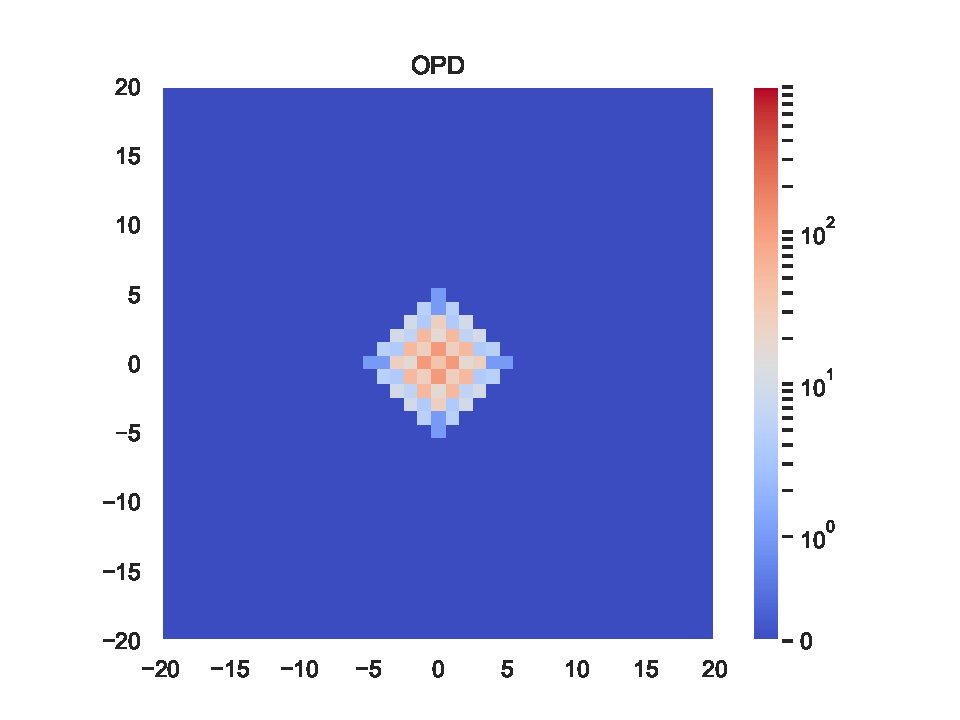
\includegraphics[trim={1.8cm 0.4cm 1.8cm 0.7cm}, clip, width=0.43\linewidth]{img/occupations_OPD.pdf}
		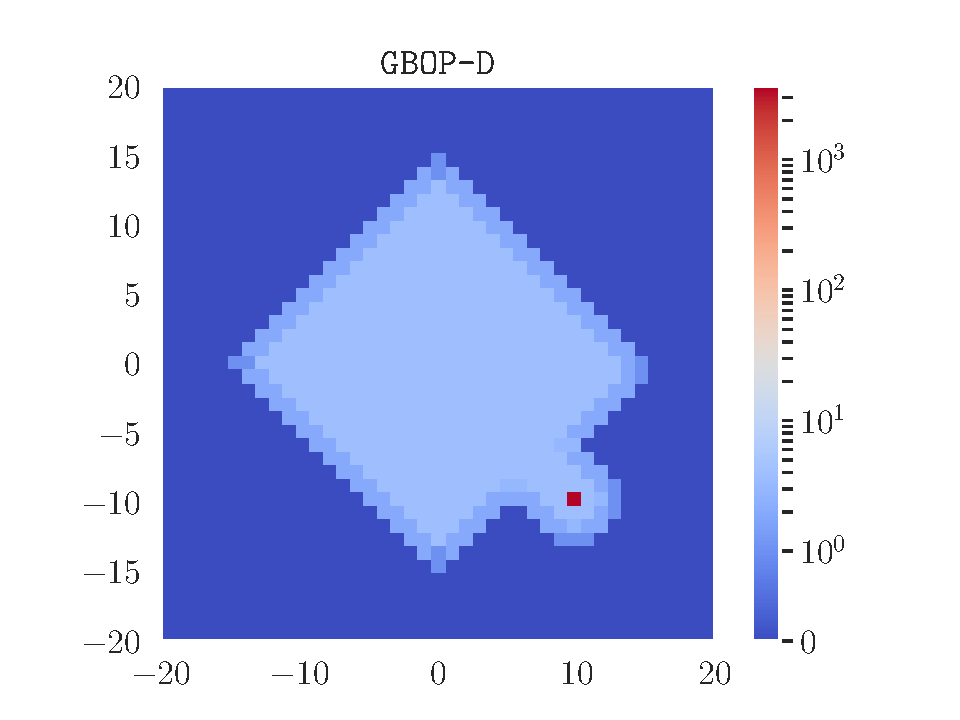
\includegraphics[trim={1.8cm 0.4cm 1.8cm 0.7cm}, clip, width=0.43\linewidth]{img/occupations_GBOP-D.pdf}
		\label{fig:deterministic-gridworld}
	}
	\subfigure[State occupancies in a stochastic gridworld.]{
		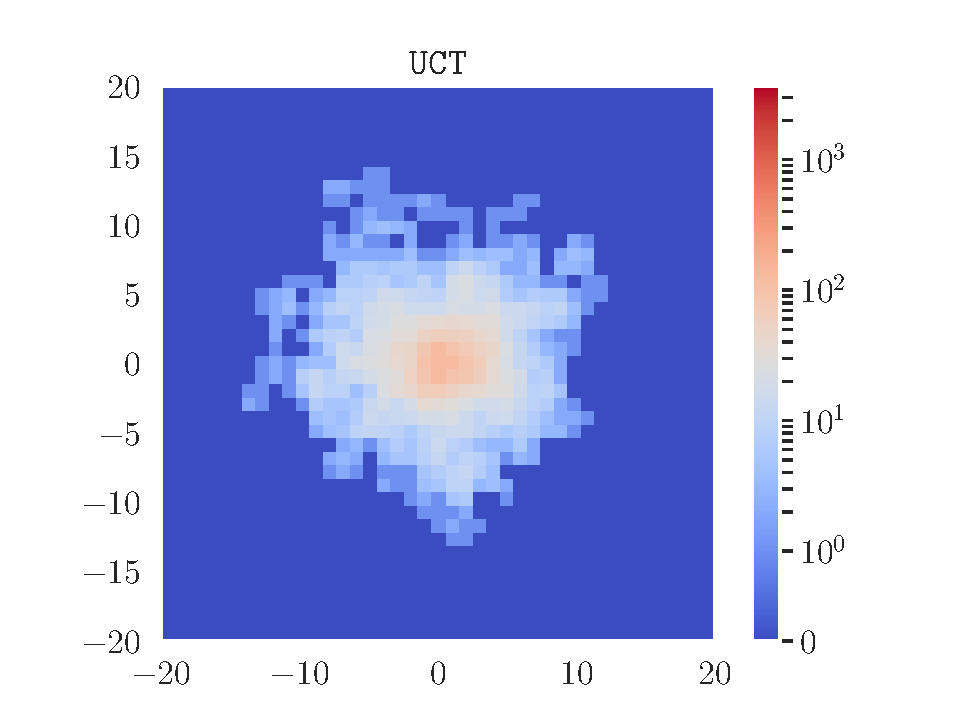
\includegraphics[trim={1.8cm 0.4cm 1.8cm 0.7cm}, clip, width=0.43\linewidth]{img/occupations_UCT.pdf}
		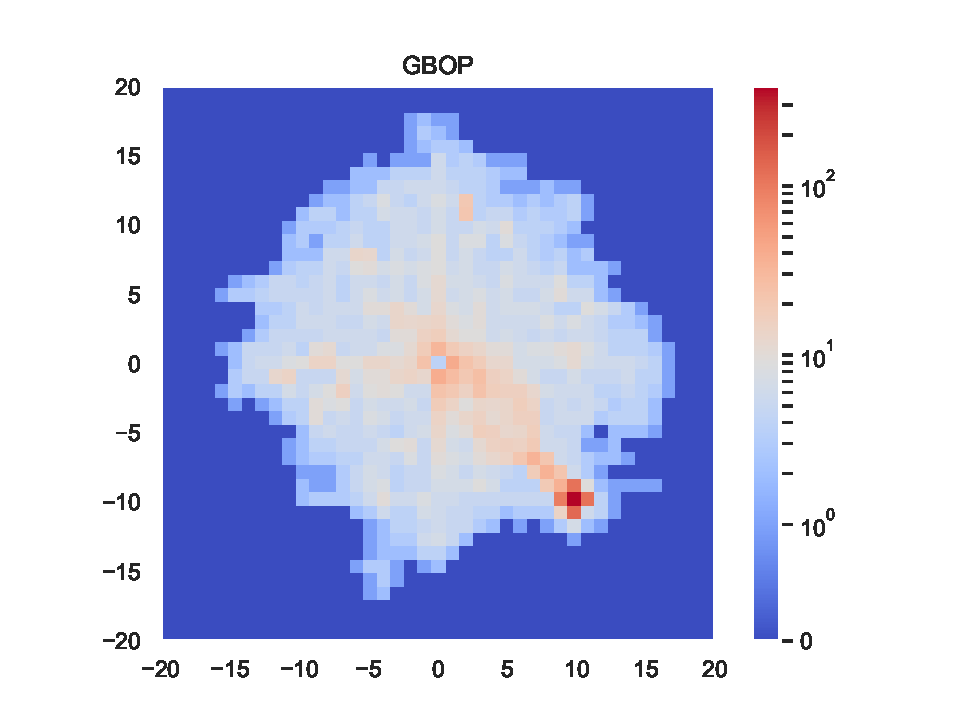
\includegraphics[trim={1.8cm 0.4cm 1.8cm 0.7cm}, clip, width=0.43\linewidth]{img/occupations_GBOP.pdf}
		\label{fig:stochastic-gridworld}
	}
\end{figure}

\paragraph{Gridworld domain.}
We consider a grid in which the agent starts at $(0,0)$ and can move in $K=4$ directions. The reward function is $0$ everywhere, except in the vicinity of a goal located at $(10, 10)$, around which the reward decreases quadratically from $1$ to $0$ in a ball of radius $5$. %: $r(x, y) = \max(1 - \frac{1}{5^2}((x-10)^2 + (y-10)^2), 0)$. 
The \Cref{fig:deterministic-gridworld} shows number of times a state is sampled by \OPD and \GBOPD, both run with a budget $n = 5460$ and discount $\gamma=0.95$. In the absence of rewards, \OPD samples sequences of actions uniformly (in a breadth-first search manner), which --because of the dynamics structure-- results in a non-uniform occupancy of the state space $S$, where the trajectories concentrate near the starting state. In contrast, \GBOPD explores uniformly in $S$, sampling each state up to four times (from its four  neighbours), until it finds the goal vicinity and finally samples the goal location indefinitely. We reproduce the experiment in the stochastic setting by adding noise on the transitions with probability $p=10\%$, and comparing \GBOP to \texttt{UCT} as we show in \Cref{fig:stochastic-gridworld}. To quantify these qualitative differences, we define in \Cref{fig:exploration} an exploration score: the mean distance $d(s_t, s_0)$ of sampled states to the initial state (exploration) minus the distance $d(s_t, s_g)$ to the goal state (exploitation).

\begin{figure}[ht]
	\centering
	\subfigure[Exploration scores in the gridworld domains.]{
		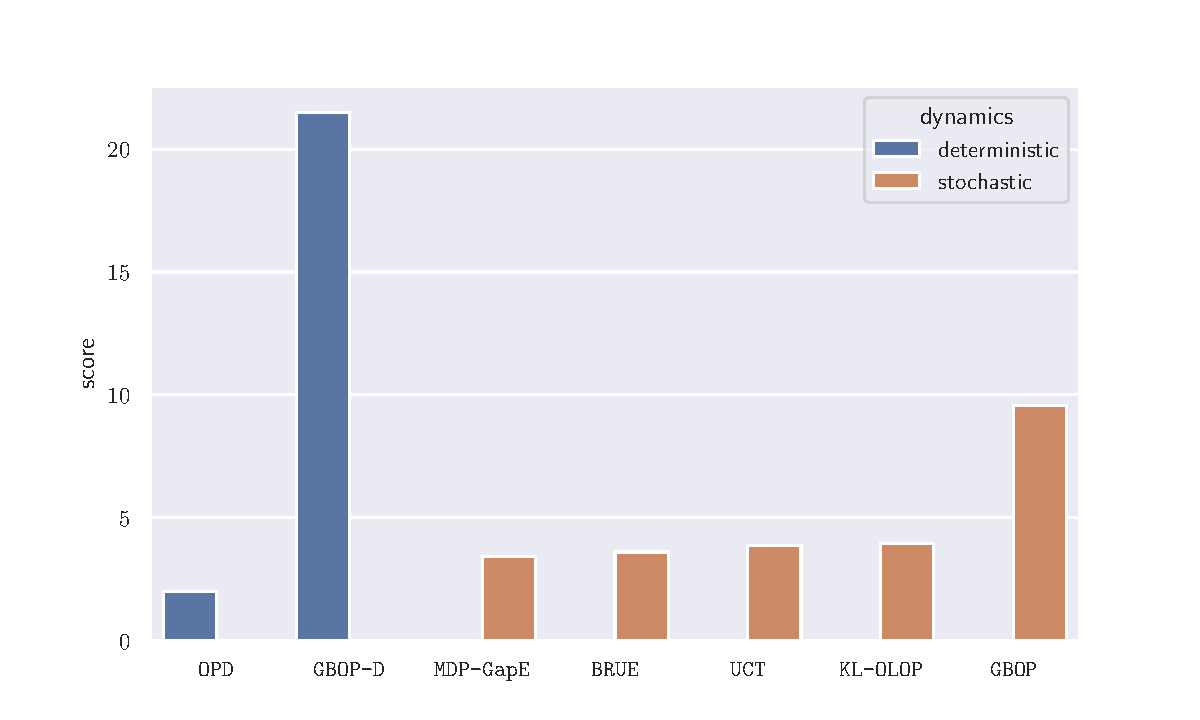
\includegraphics[trim = {1.6cm 0.cm 2cm 1.5cm}, clip, width=0.47\linewidth]{img/score.pdf}
		\label{fig:exploration}
	}
	\subfigure[Simple regret $r_n$ in the sailing domain.]{
		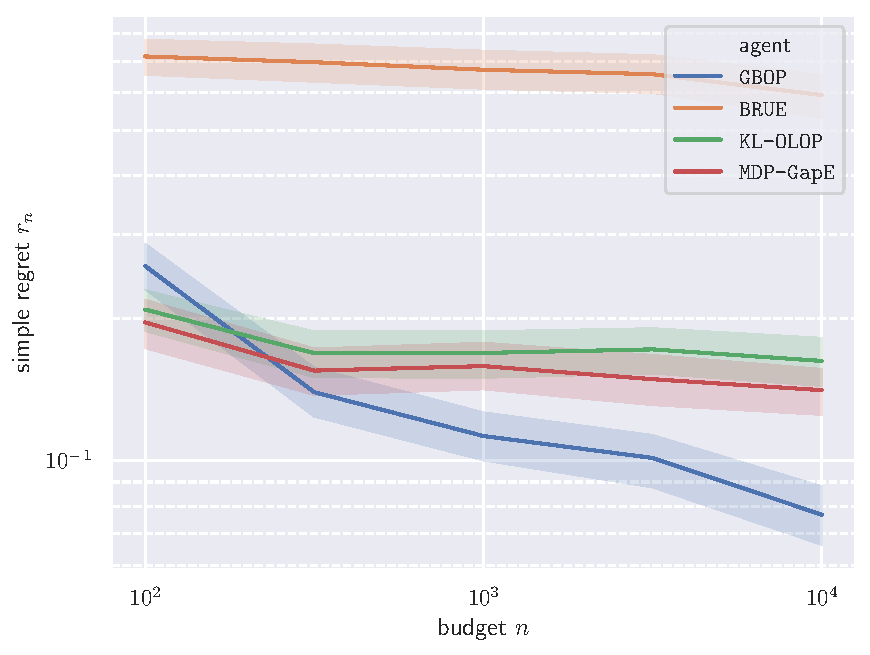
\includegraphics[trim = {0.2cm 0.2cm 0.7cm 0.5cm}, clip, width=0.4\linewidth]{img/simple_regret.pdf}
		\label{fig:sailing}
	}
	\caption{Benchmark of planning performances.}
\end{figure}


\paragraph{Sailing domain \citep{Vanderbei1996}.}
In a second experiment, a boat is sailing in $K=8$ directions to reach a goal, and suffers a cost (move duration) that depends on the direction of the wind which follows stochastic dynamics. \Cref{fig:sailing} shows the evolution of the simple regret $r_n$ of stochastic planning algorithms with respect to the number $n$ of oracle calls. We compute the mean regret and its 95\% confidence interval over 500 simulations. The asymptotic log-log slope $\sigma$ provides an empirical measurement of the effective branching factor $\kappa_e = \exp(-\log(1/\gamma)/\sigma)$ for each algorithm. We measure that %for $n>10^{3.5}$, 
$\sigma \approx-0.04$ and $\kappa_e \approx 3.6$ for \texttt{BRUE}, \texttt{KL-OLOP}, \texttt{MDP-GapE}, \texttt{UCT}. In contrast, we measure $\sigma \approx-0.3$ and $\kappa_e \approx 1.2$ for \GBOP, which suggests that our result of \Cref{thm:regret-gbop} might generalize to the stochastic setting. Additional experimental results and details are provided in the Supplementary Material.

\section*{Acknowledgement}

This work was supported by the French Ministry of Higher Education and Research, and CPER Nord-Pas de Calais/FEDER DATA Advanced data science and technologies 2015-2020.
We thank Mathieu Seurin and {\'E}milie Kaufmann for the helpful discussions and proofreading.

\FloatBarrier
\section*{Conclusion}

In this paper, we study a simple yet highly effective variant of the tree-based planning strategies. We prove that leveraging the graph structure induced by states provides a benefit over tree-based algorithms, in the form of an improved regret bound in the deterministic setting, that depends on a smaller difficulty measure. This translates into an enhanced performance in practice, and can be adapted to stochastic planning problems as we show empirically. We believe that revisiting the heart of the MCTS strategy to take into account a graph structure opens exciting novel research directions.

\bibliography{references}



%\begin{comment}
\appendix
\clearpage
\begin{center}
	\LARGE Supplementary Material
\end{center}

\paragraph{Outline}
In \Cref{sec:proof}, we provide a proof for every novel result introduced in this paper. \Cref{sec:implementation} gives additional insights about the implementation of \GBOPD and \GBOP, namely an approximation that guarantees finite-time termination and associated time-complexity. Finally, \Cref{sec:experimental-details} provides additional details about our experiments.

\section{Proofs}
\label{sec:proof}

\subsection{Proof of Lemma \ref{lem:properties-b-tree}}
\begin{proof}
The tightening property is directly obtained by definition of monotonicity.
Let us show the preservation of monotonicity. Let $U$ a monotonic upper-bound, $a\in A^h$. Then, for any $b\in A$:
\begin{align*}
U(ab) \geq B(U)(ab) \implies 
r(ab) + \gamma U(ab) \geq r(ab) + \gamma B(U)(ab).
\end{align*}
Thus, my taking the $\max$ on $b$,
$
B(U)(a) \geq B^2(U)(a).
$
The same can be obtained for a lower-bound $L$.

The finite time convergence can be obtained by recursion from the leaves to the root, by noticing that if the value of a set of siblings $aA$ is invariant by $B$, then the value of their parent $a$ is invariant by $B^2$.
\end{proof}

\subsection{Proof of Lemma \ref{lem:properties-b-graph}}
\begin{proof}
The proof of tightening and monotonicity preservation is the same as that of Lemma \ref{lem:properties-b-tree}.
The contraction property is standard for the Bellman Operator, see e.g. Puterman M., Markov Decision Processes: Discrete Stochastic Dynamic Programming (2005).
\end{proof}

\subsection{Proof of \Cref{thm:regret-opd}}
We recall the main steps of the proof of \citet{Hren2008optimistic}.\\

\begin{enumerate}
	\item The recommendation $a_n$ has a maximal depth $d_n$ in the tree, and its gap $r_n = V^\star - V({a_{n,1}})$ is bounded by $r_n \leq \frac{\gamma^{d_n}}{1-\gamma}$. We need to relate $d_n$ to $n$.
	
	\item Each expanded node belongs to $\Tau^\infty = \bigcup_{h\geq 0} \Tau_h^\infty$, where $$\Tau_h^\infty = \left\{a\in A^h: V^\star-V(a) \leq \frac{\gamma^h}{1-\gamma}\right\}.$$ Introduce the difficulty measure $\kappa$ such that $|\Tau_h^\infty| = \cO(\kappa^h)$ (the smallest).
	
	\item In the worst case, expanded nodes fully fill the depths of $\Tau^\infty$ up to $d_n$: $n = \sum_{d=1}^{d_n} n_d \leq  C\sum_{d=1}^{d_n} \kappa^d = \begin{cases}
	\cO(d_n) &\text{if $\kappa=1$}\\
	\cO(\kappa^{d_n}) &\text{else.}
	\end{cases}$\\
	Hence $r_n = \begin{cases}
	\cO(\gamma^n) &\text{if $\kappa=1$}\\
	\cO(\gamma^{\frac{\log n}{\log \kappa}}) = \cO(n^{-\frac{\log 1/\gamma}{\log \kappa}}) &\text{else.}
	\end{cases}$
\end{enumerate}

\subsection{Proof of Lemma \ref{lem:shrink}}

\begin{proof}
Let $L_2\leq L_1\leq V\leq U_1\leq U_2$, then $\Tau_h^\infty(L_1,U_1) \subset \Tau_h^\infty(L_2,U_2)$, which implies $|\Tau_h^\infty(L_1,U_1)|^{1/h} \leq |\Tau_h^\infty(L_2,U_2)|^{1/h}$ and the claimed result in the limit $h\rightarrow\infty$.
\end{proof}

\subsection{Proof of \Cref{thm:regret-bound-U}}
In this proof, we temporarily assume that $U=B(U)$ and $L=B(L)$. We follow the same steps as in the proof of the regret of \texttt{OPD}.

\begin{remark}
It no longer holds that $a_n$ must be of maximal depth $d_n$.  This is due to the fact the exploration bonus $\gamma^h U(a)$ is not depth-wise constant: consider two nodes $a,b$ at the same depth with $R(a) > R(b)$. In \texttt{OPD}, both get the same bonus $\gamma^h/(1-\gamma)$, and the node $a$ is expanded first. But with the local bonus, $b$ could be expanded in priority rather than $a$, if its own bonus is sufficiently higher than that of $a$, precisely if $R(a)+\gamma^h U(a) < R(b)+\gamma^h U(b)$. For instance, $U(a)=0$ when $a$ is known to be a terminal state while $b$ can lead to future rewards. If after expanding and exploring the subtree of $b$ we find out that $V(b) = 0$, we still return the recommendation $a$, which is of non-maximal depth.
\end{remark}

The regret bound still holds, however. First, notice that:
\begin{lemma}[Expansion]
\label{lem:expansion-bound-U}
Whenever a node $a$ of depth $h$ is expanded by the optimistic algorithm, its first action $a_1$ enjoys a simple regret $V(a^\star)-V(a_1) \leq \gamma^h(U(a)-L(a))$. 
\end{lemma}
\begin{proof}
Let $t$ be the time of expansion of $a$, it holds that $\overline{U}_t(b) \leq \overline{U}_t(a)$ for all $b\in \ext{\Tau}_t$, in particular those in a branch starting by an optimal action $a^\star$. Since $U=B(U)$ and $L=B(L)$, we also have $\overline{U}_t(a^\star) = \max_{b\in a^\star A^*} \overline{U}_t(b) \leq \overline{U}_t(a)$, and $\overline{L}_t(a_1) = \max{b\in a_1 A^*} \overline{L}_t(b) \geq  \overline{L}_t(a)$. Thus, $V(a^\star)-V(a_1) \leq \overline{U}_t(a^\star) - \overline{L}_t(a_1) \leq \overline{U}_t(a) - \overline{L}_t(a) = \gamma^h(U(a)-L(a))$.
\qed\end{proof}
 
\begin{lemma}[Recommendation]
	\label{lem:recommendation-bound-U}
The recommended action $a_n$ has a simple regret $r_n \leq \frac{\gamma^{d_n}}{1-\gamma}$, where $d_n$ is the maximal depth of $\Tau_n$.
\end{lemma}
\begin{proof}
Let $i$ a node of maximal depth $d_n$, and consider the recommended node $a_n$ at time $n$, of depth $d$. In particular, $\overline{L}_n(a_n) \geq \overline{L}_n(i)$, and since $(\overline{L}_t)_t$ is non-decreasing we also have $\overline{L}_n(i) \geq \overline{L}_t(i)$. At the time $t$ when $i$ is expanded, we have $\overline{U}_t(a_n) \leq \overline{U}_t(i)$, and since $(\overline{U}_t)_t$ is non-increasing we also have $\overline{U}_n(a_n) \leq \overline{U}_t(a_n)$. We can conclude with Lemma \ref{lem:expansion-bound-U} applied to $a_n$: $r_n \leq \gamma^d(U(a_n)-L(a_n) = \overline{U}_n(a_n) - \overline{L}_n(a_n)  \leq \overline{U}_t(a_n) - \overline{L}_n(i) \leq \overline{U}_t(i) - \overline{L}_t(i) = \gamma^{d_n}(U(i) - L(i)$, which yields the claimed bound since $U(i) - L(i) \leq V_{\max}-0$.
\qed\end{proof}

\begin{lemma}[Near-optimal nodes]
\label{lem:near-optimal-nodes-U}
Every node expanded by \eqref{eq:sampling_rule} is in $\Tau^\infty(L,U) = \bigcup_{h\geq 0} \Tau^\infty_h(L,U)$.
\end{lemma}
\begin{proof}
Let $a$ be a node of depth $h$ expanded at round $n$, then $\overline{U}_n(a) \geq \overline{U}_n(b)$ for all $b\in\ext{\Tau}_n$. Thus, since $U = B(U)$, we have $\overline{U}(a) = \overline{B(U)}(\emptyset) = B(U)(s_0) \geq V(s_0) = V^\star$. Thus, $V^\star - V(a) \leq \overline{U}(a) - \overline{L}(a) = \gamma^h(U(a) - L(a))$.
\qed\end{proof}

Finally, we can move on to the proof of \Cref{thm:regret-bound-U}.
Let $n_d$ be the number of expanded nodes of depth $d$, by Lemma \ref{lem:near-optimal-nodes-U} we have $n_d \leq |\Tau^\infty_d(L,U)| \leq C\kappa(L,U)^d$. Thus, 
\[n = \sum_{d=1}^{d_n} n_d \leq C\sum_{d=0}^{d_n} \kappa(L,U)^d = C\frac{\kappa(L,U)^{d_n+1}-1}{\kappa(L,U)-1}\]
Hence, $d_n \geq C'\frac{\log n}{\log\kappa(L,U)},$ which along with Lemma \ref{lem:expansion-bound-U} gives the claimed bound.

Note that if $L,\,U$ are monotonic bounds that do not verify $L = B(L)$ and $U=B(U)$, then planning with $B(L),B(U)$ instead will yield the proved bound with a branching factor $\kappa(B(L),B(U))$, and since $L\leq B(L)\leq V\leq B(U)\leq U$ we have $\kappa(B(L),B(U)) \leq \kappa(L,U)$, which still gives \begin{align*}
r_n = \cO\left(n^{-\frac{\log 1/\gamma}{\log \kappa(L,U)}}\right);
\end{align*}

%\subsection{Proof of Proposition \ref{prop:b-eq-mb}}

%\begin{proof}
%	Let $U$ equivalent to $\cU$, and $a\in T_n$.
%	If $a\in\ext{T_n}$, then necessarily $s(a)\in\ext{\cG_n}$, and both are unchanged by $B_n$ and $\cB_n$ respectively.
%	If $a\in\inte{T_n}$, then necessarily $s(a)\in\int{\cG_n}$. There exist a'
%\qed\end{proof}

%\subsection{Proof of Lemma \ref{lem:properties-mb}}
%\begin{proof}
%Let $U_1, U_2\in \Real^\Tau_n, a\in\Tau_n$,
%\begin{align*}
%    (M_n^+ U_1 - M_n^+ U_2)(a) &= \min_{a'\in N_n(a)} U_1(a') - \min_{a'\in N_n(a)} U_2(a') \\
%    &= \min_{a'\in N_n(a)} U_1(a') - U_2(a^-) \\
%    &\leq U_1(a^-) - U_2(a^-) \\
%    &\leq \|U_1 - U_2\|_\infty
%\end{align*}
%where $a^-\in \argmin_{a'\in N_n(a)} U_2(a')$. 
%Hence, $\|M_n^+ U_1 - M_n^+ U_2\|_\infty \leq \|U_1 - U_2\|_\infty$
%\qed\end{proof}
%
%\subsection{Proof of Proposition \ref{prop:pruning}}
%
%\begin{proof}
%Assume $h(a_2) \geq h(a_1)$.
%\begin{align*}
%    V(a_1) - V(a_2) &= R(a_1)- R(a_2) + \underbrace{\left(\gamma^{h(a_1)} - \gamma^{h(a_2)}\right)}_{\geq 0}V(s) \\
%    &\leq R(a_1)- R(a_2) + \left(\gamma^{h(a_1)} - \gamma^{h(a_2)}\right)U(s)\\
%    &= \overline{U}(a_1) - \overline{U}(a_2)
%\end{align*}
%Hence, if this last term is negative, then $V(a_1) - V(a_2)$ is as well.
%\qed\end{proof}

\subsection{Proof of Lemma \ref{lem:equivalence}}
\begin{proof}
	
We first show that if $U$ is equivalent to $\cU$, meaning that for any sequence $a\in T(\cG_n)$ we have $U(a) = \cU(s(a))$, then $B_n(U)$ is equivalent to $\cB_n(\cU)$.

By definition of $T(\cG_n)$, any sequence of action $a\in T(\cG_n)$ corresponds to a path $s_0, a_0,\dots, s_{h-1}, a_{h-1}, s_{h}$ in $\cG_n$. If $a\in\ext{T(\cG_n)}$, then necessarily $s(a)\in\ext{\cG_n}$, and both are unchanged by $B_n$ and $\cB_n$ respectively. Conversely, if $a\in\inte{T}(\cG_n)$, then $s(a)\in\inte{\cG_n}$ by construction. Thus, $B_n(U)(a) = \max_{b\in A} r(s(a), b) + \gamma U({ab}) = \max_{b\in A} r(s(a), b) + \gamma \cU(s({ab}))$ (by hypothesis) $= \max_{b\in A} r(s(a), b) + \gamma \cU(P(s({a}),b)) = \cB_n(\cU_n)(s(a))$.

By induction, for any $k>0$ $B_n^k(U)$ is equivalent to $\cB_n^k(\cU)$, and at the limit $k\rightarrow\infty$ it comes that $U_n$ is equivalent to $\cU_n$. The same result can be shown similary for $L_n$ and $\cL_n$.
\qed\end{proof}

\subsection{Proof of Lemma \ref{lem:expansion-bound}}

We start by showing a preliminary lemma.
\begin{lemma}[Bounds of sequence values]
	\label{lem:bounds}
	The bounds $(\overline{L}_n, \overline{U}_n)$ on the value of sequences of actions verify are respectively non-decreasing and non-increasing with respect to $n$, and verify: for all $a\in A^*$, $\overline{U_n}(a) = \max_{a'\in a A^\infty} \overline{U}(a')$.
\end{lemma}
\begin{proof}
	The second property can be easily shown by induction using the fact that $U_n$ and $L_n$ are fixed-points of $B_n$ by definition. Applying this equation at each depth $h$ gives the result. From this observation, we can deduce that $\overline{L}_n$ is increasing with $n$. Indeed, since when $T(\cG_n)$ is expanded with additional nodes compared to $T(\cG_{n-1})$, the leaves $a$ of $T(\cG_{n-1})$ with previous value $L_{n-1}(a)=0$ are updated to $L_n(a) = \max_b r(s(a), b) \geq 0 = L_{n-1}(a)$, and this increase at the leaves is then propagated through $\max_{a'\in a A^\infty}$ to any internal node $a$. Thus, $L_n$ is non-decreasing and likewise, $U_n$ is non-increasing with respect to $n$. The same is obtained directly of the bounds on sequence values $(\overline{L}_n, \overline{U}_n)$.
\qed\end{proof}

Which enables us to proceed to the proof of Lemma \ref{lem:expansion-bound}.
\begin{proof}
	Let $t$ be the time of expansion of $a$, it holds that $\overline{U}_t(b) \leq \overline{U}_t(a)$ for all $b\in T(\cG_n)$. In particular for $b$ in a branch starting by an optimal action $a^\star$ $\overline{U}_t(a) \geq \max_{b\in a^\star A^*}  \overline{U}_t(b) = \overline{U}_t(a^\star)$. Thus, $V(a^\star)-V(a) \leq \overline{U}_t(a^\star) - \overline{L}_t(a) \leq \overline{U}_t(a) - \overline{L}_t(a) = \gamma^h(U_t(a)-L_t(a))$.
\qed\end{proof}

\subsection{Proof of Lemma \ref{lem:recommendation-bound}}
\begin{proof}
	Let $i$ an expanded node of maximal depth $d_n\in\Real\cup\{\infty\}$, and consider the recommended node $a_n$ at time $n$, of depth $d\in\Real\cup\{\infty\}$. In particular, $\overline{L}_n(a_n) \geq \overline{L}_n(i)$, and since $(\overline{L}_t)_t$ is non-decreasing we also have $\overline{L}_n(i) \geq \overline{L}_t(i)$. At the time $t$ when $i$ is expanded, we have $\overline{U}_t(a_n) \leq \overline{U}_t(i)$, and since $(\overline{U}_t)_t$ is non-increasing we also have $\overline{U}_n(a_n) \leq \overline{U}_t(a_n)$. We can conclude with Lemma \ref{lem:expansion-bound} applied to $a_n$: $r_n \leq V^\star - V(a_n) \leq  \gamma^d(U(a_n)-L(a_n) = \overline{U}_n(a_n) - \overline{L}_n(a_n)  \leq \overline{U}_t(a_n) - \overline{L}_n(i) \leq \overline{U}_t(i) - \overline{L}_t(i) = \gamma^{d_n}(U_t(i) - L_t(i)$, which yields the claimed bound since $U(i) - L(i) \leq V_{\max}-0$.
\qed\end{proof}


\subsection{Proof of \Cref{thm:regret-gbop}}

\begin{proof}
Let $\kappa'>\kappa_\infty$. Since $\kappa(L_n,U_n)\rightarrow\kappa_\infty$, there exists $n_0\in\Natural$ such that for all $n\geq n_0$, $\kappa(L_n,U_n) \leq \kappa'$.
By Lemma \ref{lem:expansion-bound}, at each iteration $n$ the expanded node must belong to $\Tau^\infty(L_n,U_n)$.
Let $n\geq n_0$, and define $d_0 = \min\{d\in\Natural: \exists t \in[n_0,n], b_t\in A^d \}$. By definition, for all $d\geq d_0$, any expanded node of depth $d$ was expanded at a time $t\geq n_0$, and thus $b_t\in\Tau^\infty_t \subset\Tau^\infty_{n_0}$. We denote $n_d$ the number of expanded nodes of depth $d$. If $d_n=\infty$,then $r_n = 0$ and the bound holds. Else, we obtain
\[
n = \sum_{d=0}^{d_0-1}n_d + \sum_{d=d_0}^{d_n} n_d \leq  C_0 + C_1\sum_{d=d_0}^{d_n} (\kappa')^d \leq C_0 + C_1' (\kappa')^{d_n}
\]
And since $r_n \leq \frac{\gamma^{d_n}}{1-\gamma}$ by Lemma \ref{lem:recommendation-bound}, we obtain the claimed bound.

Moreover, given a history of observed transitions up to iteration $n$, the bounds $U_n, L_n$ obtained from \eqref{eq:gbop-t-bounds} on the unrolled tree $T(\cG_n)$ are tighter than those of \eqref{eq:opd-bounds} since $T_n\subset T(\cG_n)$, which implies by Lemma \ref{lem:shrink} that $\kappa(L_n, U_n) \leq \kappa$. We obtain $\kappa_\infty \leq \kappa$ at the limit. 
\qed\end{proof}

\subsection{Proof of Proposition \ref{prop:illustrative-example}}

The \Cref{fig:mdp-tree} shows the planning tree corresponding to the MDP $\cM$. Whenever the action $a_1$ is taken \textcolor{green}{(in green)} the resulting subtree is represented by a leaf node $s^\star$ of value $V^\star = \frac{r^\star}{1-\gamma}$. When, in contrast, we take a sequence of actions among $a_2\dots a_K$ \textcolor{red}{(in red)}, we stay in the state $s^+$ and denote $V_h$ the corresponding value at depth $h$.

\begin{figure}
    \centering
    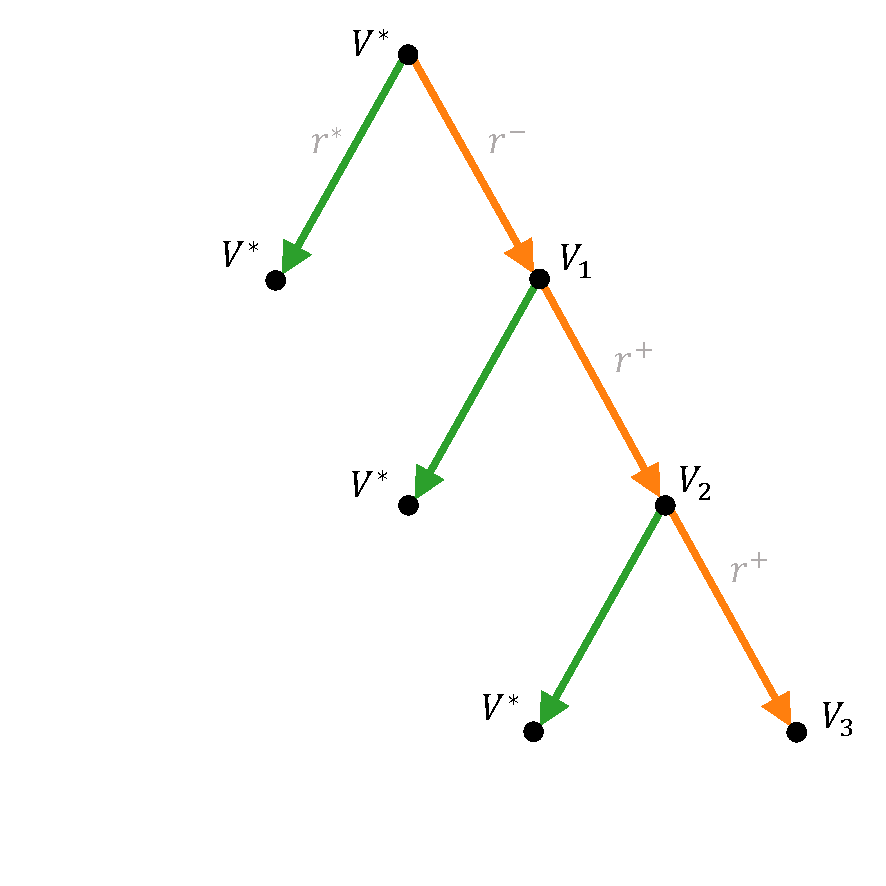
\includegraphics[trim={3.5cm 2cm 0.5cm 0.5cm}, clip, width=0.5\linewidth]{img/mdp_tree.pdf}
    \caption{Planning tree of the MDP $\cM$ of \Cref{fig:mdp}}.
    \label{fig:mdp-tree}
\end{figure}
\begin{lemma}
 Any sequence of actions in $A\setminus{a_1}$ is in $\Tau^\infty$.
\end{lemma}
\begin{proof}
Any such sequence of actions yields the sequence of rewards $r^-, r^+, \dots,r^+$. and end up in the state $s^+$ with value at least $V^\star$ (obtained by further taking $a_1$ indefinitely). Thus its value $V_h$ verifies, 
\begin{align*}
    V_h &\geq \sum_{t=0}^{h-1} \gamma^t r_t + \gamma^h V^\star\\
    &= r^- - r^+ + \sum_{t=0}^{h-1} \gamma^t r^+ + \gamma^h V^\star \\
    &= (-\frac{\gamma}{1-\gamma} - 1)S + \frac{1-\gamma^h}{1-\gamma} (r^\star + S) + \gamma^h V^\star\\
    &= V^\star - S\frac{\gamma^h}{1-\gamma} \geq V^\star - \frac{\gamma^h}{1-\gamma}
\end{align*}
\qed\end{proof}

We can directly conclude that $\kappa \geq \limsup{|\{a_2,\dots,a_K\}^h|^{1/h}} = K-1$.

Now, consider the nodes expanded by \GBOPD. The first expansion is that of the root, which discovers $s^\star$ and $s^+$. In the absence of information on these two state, the bound $V_{\max}$ is used and the first action $a_1$ gets a higher $\overline{U}$ that any other action $a_2,\dots,a_K$ since $r^\star \geq r^-$. Hence, at the second iteration, the node $a_1$ gets expanded. At this point, the self-loop of the state $s^\star$ is discovered, which means that form now on the bounds verify $L_n(a_1) = V^\star = U_n(a_1)$ for $n\geq2$, which means that $L_n(a_1A^*)-U_n(a_1A^*) = 0$. The nodes $a_2,\dots,a_K$ can be expanded at most once before the entire MDP is discovered and $L_n=V=U_n$ over the entire tree, which means that $\Tau_n^\infty$ is the set of optimal nodes, i.e. the nodes in the only optimal sequence $a_1^\star$. Hence, $\kappa_\infty = 1.$ 

\section{Implementation Details}
\label{sec:implementation}

In this section, we provide more details about the implementation of \GBOPD and \GBOP. First, we discuss how two procedures can be approximated so that they terminate in finite time, and study the impact of this approximation on the regret guarantees. Second, we propose a lazy implementation of the bounds computation through $\cB_n^\infty$ that only considers a subset of nodes to update.

\subsection{Termination}

\subsubsection{Bounds computation}

The bounds computation step $\cB_n^\infty$ (line 1 of \GBOPD) can converge in infinite time whenever $\cG_n$ contains a loop, as shown in \Cref{fig:simple_loop}. We consider the effect of stopping early after a fixed number of iterations $k(\varepsilon,\gamma)$.

\begin{figure}[th]
	\centering
	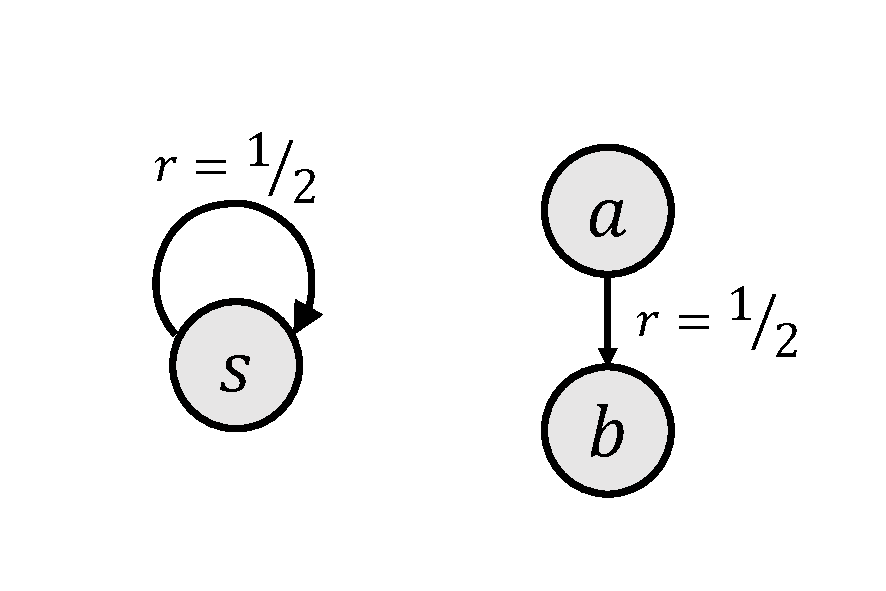
\includegraphics[trim=2.5cm 1cm 9cm 2cm, clip, width=0.1\linewidth]{img/loop.pdf}\\
	\begin{tabular}{lccccc}
		\toprule
		$k$ & $0$ & $1$ & $\cdots$ & $k$ \\
		\midrule
		$\cU = \cB^k(V_{\max})(s)$ & $V_{\max}$ & $\frac{1}{2} + \gamma V_{\max}$ && $\frac{1}{2}(1-\gamma^k)V_{\max} + \gamma^k V_{\max}$\\
		$\cL = \cB^k(0)(s)$ & $0$ & $\frac{1}{2}$ && $\frac{1}{2}(1-\gamma^k)V_{\max}$\\
		\bottomrule
	\end{tabular}
	\caption{\textbf{Top}: a simple looping MDP with $|S|=|A|=1$ after having observed a single transition ($n=1$). \textbf{Bottom}: the sequence of bounds $\cB_1^k(0)$ and $\cB_1^k(V_{\max})$. They converge geometrically to their limit $\cU_1 = \cL_1 = V = \frac{1}{2}V_{\max}$, thus in infinite time.}
	\label{fig:simple_loop}
\end{figure}

\begin{proposition}[Time complexity of bounds computation]
An $\varepsilon$-approximation of $(\cL_n, \cU_n)$ can be computed by applying $\cB_n$ for a finite number $k(\epsilon,\gamma)$ of iterations, with $$k(\epsilon,\gamma) = \log_\gamma\frac{1}{\varepsilon(1-\gamma)}.$$ 
\end{proposition}
\begin{proof}
	$\cB_n$ is a $\gamma$-contraction by Lemma \ref{lem:properties-b-graph}, and $\cU_n$ (resp $\cL_n$) is at a distance (in $\|\dot\|_\infty$) at most $V_{\max}$ of the initial value bound $V_{\max}$ (resp $0$). Thus, the $k^{\text{th}}$ application of $\cB_n$ decreases this error by a factor $\gamma^k$, which gives the result.
\qed\end{proof}

The impact of using an $\varepsilon$-approximation of $(\cL_n, \cU_n)$ during planning is the following:
\begin{proposition}[Effect of early stopping]
	\label{prop:early-stopping}
Denote the approximate bounds $(\hat{\cL}_n, \hat{\cU}_n)$ obtained by applying $\cB_n^{k(\varepsilon,\gamma)}$ instead of $\cB_n^\infty$, and likewise $(\hat{L}_n, \hat{U}_n)$ in their tree version obtained by applying $B_n^{k(\varepsilon,\gamma)}$ instead of $B_n^\infty$.
Then, running \GBOPD with $\hat{\cL}_n, \hat{\cU}_n$ gives the following regret:
\begin{align*}
r_n = \tilde{\cO}\left(n^{-\log \frac{1}{\gamma}/\hlob{\log \hat{\kappa}_\infty}}\right),
\end{align*}
with $$\hlgb{{\kappa}_\infty} \leq \hlob{\hat{\kappa}_\infty \eqdef \lim_{n\rightarrow\infty} \kappa(\hat{L}_n, \hat{U}_n)} \leq \hlrb{\kappa}.$$
Moreover, the approximation gap $\hlgb{\kappa_\infty} - \hlob{\hat{\kappa}_\infty}$ is non-increasing with respect to $\varepsilon$.
\end{proposition}
It is difficult to control more explicitly the gap between $\hlgb{\kappa_\infty}$ and $\hlob{\hat{\kappa}_\infty}$, which might be discontinuous with $\varepsilon$.

\begin{proof}
	Note that $\hat{L}_n$ and $\hat{U}_n$ are valid monotonic bounds on $V$, verifying
	\[0\leq \hat{L}_n\leq {L}_n \leq V \leq {U}_n\leq \hat{U}_n \leq V_{\max}.\]
	Thus, Lemma \ref{lem:bounds} holds with the difference that we only have an inequality $\overline{U_n}(a) \geq \max_{a'\in a A^\infty} \overline{U}(a')$ rather than an equality, by monotonicity but non-invariance by $B_n$. However, this was the actual inequality used in Lemma \ref{lem:expansion-bound}, which still holds by replacing $L_n,U_n$ by their approximation $\hat{L}_n,\hat{U}_n$. Likewise, Lemma \ref{lem:recommendation-bound} holds. The proof of \Cref{thm:regret-gbop}, can be written with the modification that expanded nodes belong to $T_h^\infty(\hat{L}_n, \hat{U}_n))$, which gives the claimed bound.
	
	As $\varepsilon$ decreases, $k(\epsilon,\gamma)$ increases, which means by Lemma \ref{lem:properties-b-tree} that $(\hat{\cL}_n, \hat{\cU}_n)$ get tighter and $\hlob{\hat{\kappa}_\infty}$ shrinks by Lemma \ref{lem:shrink}. It reaches its minimum $\hlgb{\kappa_\infty}$ when $\varepsilon=0$.
\qed\end{proof}

Thus, we observe that there is a \emph{tradeoff} between the time complexity $k(\varepsilon)$ and the sample complexity $\hlob{\hat{\kappa}_\infty}$: decreasing one increases the other.

Note that \OPD uses $d_n$ iterations of $B_n$, which corresponds to a tuning of $\varepsilon$ with $n$: $\varepsilon_n = \frac{\gamma^{d_n}}{1-\gamma} = \cO(n^{-\frac{\log 1/\gamma}{\log \kappa}})$. 


\subsubsection{Sampling rule}

The sampling rule of \GBOPD (line 2 of \GBOPD) can yield an infinite sequence $b_n$. We propose to stop the sampling after a fixed depth $d^+_n$.

\begin{proposition}[Time complexity of sampling]
	Consider the variant of \GBOPD where we stop the sampling rule when reaching a fixed depth $d^+_n$ chosen polynomial with $n$:
	\[d^+_n = \ceil{\alpha n^\beta},\; \text{with }\alpha,\beta > 0\]
	Then, the regret bound of \Cref{thm:regret-gbop} (or that of Proposition \ref{prop:early-stopping} when using early stopping in the bounds computation) still holds.
\end{proposition}

Note that this is not too constraining compared to \OPD, for which the sampling rule complexity $d_n$ is upper-bounded by $n$. Hence, by choosing $\alpha=\beta=1$, \GBOPD preserve the same complexity as \OPD in the worst case.

\begin{proof}
	Let $\kappa'>\hlgb{{\kappa}_\infty}$ (or $\kappa'>\hlob{\hat{\kappa}_\infty}$ under approximate bounds). In the proof of \Cref{thm:regret-gbop}, it is shown that the maximum depth $d_n$ of an expanded node is at least $d^-_n \eqdef \log_{\kappa'}\frac{n-C_0}{C_1'}$, which allows to conclude with Lemma \ref{lem:recommendation-bound} that $r_n = \cO(\gamma^{d_n}) = \cO(\gamma^{d^-_n})$. By choosing $d^+_n$ polynomial, we have that $d^+_n$ is greater than $d^-_n$ for $n$ sufficiently high. Thus, by stopping the sampling after reaching a depth $d^+_n$, we have that $r_n \leq \gamma^{\min\{d_n, d^+_n\}} / (1-\gamma) = \cO(\gamma^{d^-_n}) = \cO(n^{\frac{-\log 1/\gamma}{\log \kappa'}})$
\qed\end{proof}

\subsection{Efficient implementation of $\cB_n^\infty$}

The bounds $\cL_n$ and $\cU_n$ are computed by fixed-point iteration of $\cB_n$ from the trivial bounds $(0,V_{\max})$. The naive implementation of $\cB_n$ requires to iterate over the whole set of state-action pairs in $\cG_n$. 
Two ideas can be used to increase the efficiency of both steps:
\begin{enumerate}[(i)]
	\item Instead of starting the iteration with the trivial bounds, the previous estimate $\cL_{n-1}, \cU_{n-1}$ can be used instead at iteration $n$. Since these bounds are closer to their limit ($0\leq \cL_{n-1}\leq \cL_n$ and $\cU_n\leq \cU_{n-1} \leq V_{\max}$), the fixed-point iteration will converge quicker.
	\item In particular, since $\cL_{n-1}$ and $\cU_{n-1}$ are invariant by $\cB_n$, the the only nodes modified by a supplementary application of $\cB_n$ are the parents of only updated node: the expanded state $s_n$. Once its value is updated by $\cB_n$, the same reasoning can be applied for the next iteration of $\cB_n$: only its predecessors can be updated. Thus, we can keep track of a set $q$ of states that can be updated, for every application of $\cB_n$.
\end{enumerate}
These idea are formalised in \Cref{alg:queue-b-inf}. Note that the criterion $\|\cB_n^{k+1} - \cB_n^k\| \leq \frac{1-\gamma}{\gamma}\varepsilon$ is used to detect that the limit $\cB_n^\infty$ is approximated with accuracy $\varepsilon$, and stems from $\cB_n$ being a $\gamma$-contraction:
\begin{proof}
$\|\cB_n^k - \cB_n^\infty\| \leq \gamma\| \cB_n^{k+1} - \cB_n^\infty\| \leq \gamma \|\cB_n^{k+1} - \cB_n^{k}\| + \gamma \|\cB_n^{k} - \cB_n^\infty\|$, with $\| \cB_n^{k+1} - \cB_n^{k}\| \leq \frac{1-\gamma}{\gamma}\varepsilon$, thus $\|\cB_n^{k} - \cB_n^\infty\| \leq \varepsilon$.
\qed\end{proof}

\begin{algorithm}
	\caption{A queue-based implementation of $\cB_n^\infty$.}
	\label{alg:queue-b-inf}
	\KwIn{Initial bound $\cU_{n-1}$, expanded node $s_n$, accuracy $\varepsilon$}
	\KwOut{An $\varepsilon$-approximation of $\cU_{n}$}
	\DontPrintSemicolon
	$\cU_n \gets \cU_{n-1}$\;
	$q\gets [s_n]$\;
	\While{$q$ is not empty}{
		$s'\gets$ Pop the first node from the queue $q$\;
		$\cU' \gets \cB_n(\cU_n)(s')$\Comment*[r]{Node backup}
		\If(\Comment*[f]{Stopping rule}){$\cU' - \cU_n > \frac{1-\gamma}{\gamma}\varepsilon$}{
			Push the predecessors $s$ of $s'$ to the queue $q$ \Comment*[r]{Propagation rule}
		}
		$\cU_n(s') \gets \cU'$\;
	}
	\Return $\cU_n$\;
\end{algorithm}

\section{Experimental Details}
\label{sec:experimental-details}

In this section, we provide additional details and results about the experiments discussed in \Cref{sec:experiments}.

\paragraph{Parameters.} In every experiment, we used $\gamma=0.95$. In \GBOPD and \GBOP, the fixed accuracy $\varepsilon=\num{1e-2}$ was used for computing $\cB_n^\infty$, and the sampling ruled was stopped after reaching the depth $d^+_n = n$ (see \Cref{sec:implementation}).
Regarding the tuning of confidence intervals in \GBOP, since the rewards are deterministic and the transitions are stochastic in both domains we used $\beta^r(n_t(s,a), n) = 0$ and $\beta^p(n_t(s,a), n) = \log n$, following the recommendations of \citep{Leurent2019practical,Jonsson2020planning}. The maximal size $B$ of the support of the transitions $P\left(s'|s,a\right)$ was also used ($B=4$ in the gridworld domain and $B=3$ in the sailing domain) to accelerate the computations of the confidence region $\cC_t$ for transitions, as explained in \citep{Jonsson2020planning}.

\paragraph{Additional results.}

We show in \Cref{fig:suppl-occupancies} some  occupancy plots for additional planning algorithms in the stochastic Gridworld domain.
In \Cref{fig:suppl-trees}, we compare the trees $T_n$ expanded by \OPD and \texttt{KL-OLOP} to the unrolled graph $T(\cG_n)$ of \GBOPD in the deterministic gridworld domain. For clarity of the figure, we only display the nodes selected for expansion and not the entire $T(\cG_n)$ as in \Cref{fig:unroll}, since it is infinite and fractal. We observe that \OPD explores uniformly in the space of sequences, which results in a concentrated exploration in the state space as seen in \Cref{fig:deterministic-gridworld}. This phenomenon is similar to the concentration properties of martingales. \texttt{KL-OLOP} behaves similarly, but allocates its bugdet $n$ in fewer trajectories of higher length than \OPD, which results in a sparser tree and slightly better exploration (compare \Cref{fig:deterministic-gridworld} to \Cref{fig:suppl-occupancies}). In contrast, \GBOPD expands a very sparse and unbalanced tree $T(\cG_n)$ which corresponds to uniform exploration in the state space, and allows to explore deeper for the same budget $n$ (The tree is only shown up to depth $12$, but continues much deeper since the optimal transition is sampled indefinitely once it is discovered). In particular, the paths towards the goal are sampled many times, while other algorithms are still balanced at the root in terms of number of visits.

\begin{figure}[th]
	\centering
	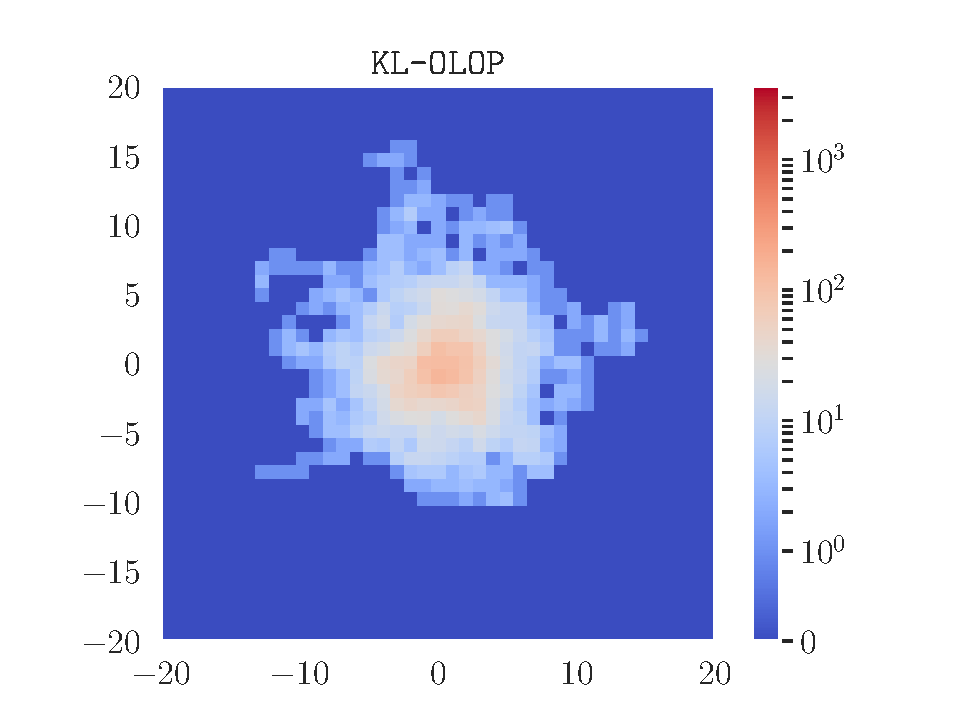
\includegraphics[trim={1.8cm 0.7cm 1.8cm 0.7cm}, clip, width=0.49\linewidth]{img/occupations_KL-OLOP.pdf}
	\hfill
	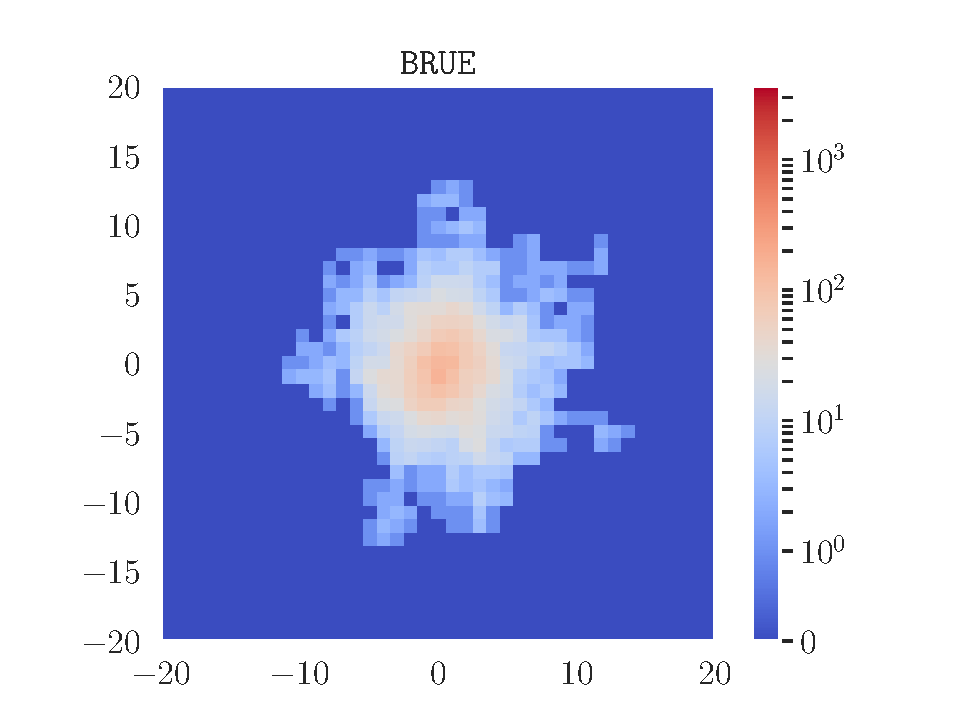
\includegraphics[trim={1.8cm 0.7cm 1.8cm 0.7cm}, clip, width=0.49\linewidth]{img/occupations_BRUE.pdf}\\
	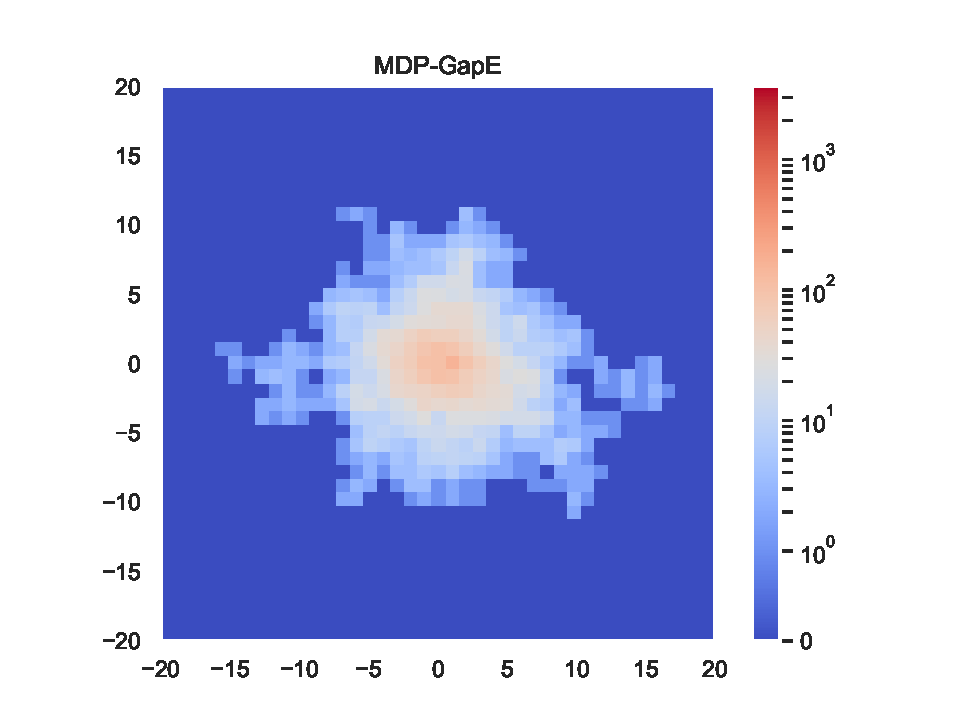
\includegraphics[trim={1.8cm 0.7cm 1.8cm 0.7cm}, clip, width=0.49\linewidth]{img/occupations_MDP-GapE.pdf}
	\caption{State occupancies of other planning algorithms in a stochastic gridworld.}
	\label{fig:suppl-occupancies}
\end{figure}


\begin{figure}[tp]
	\centering
	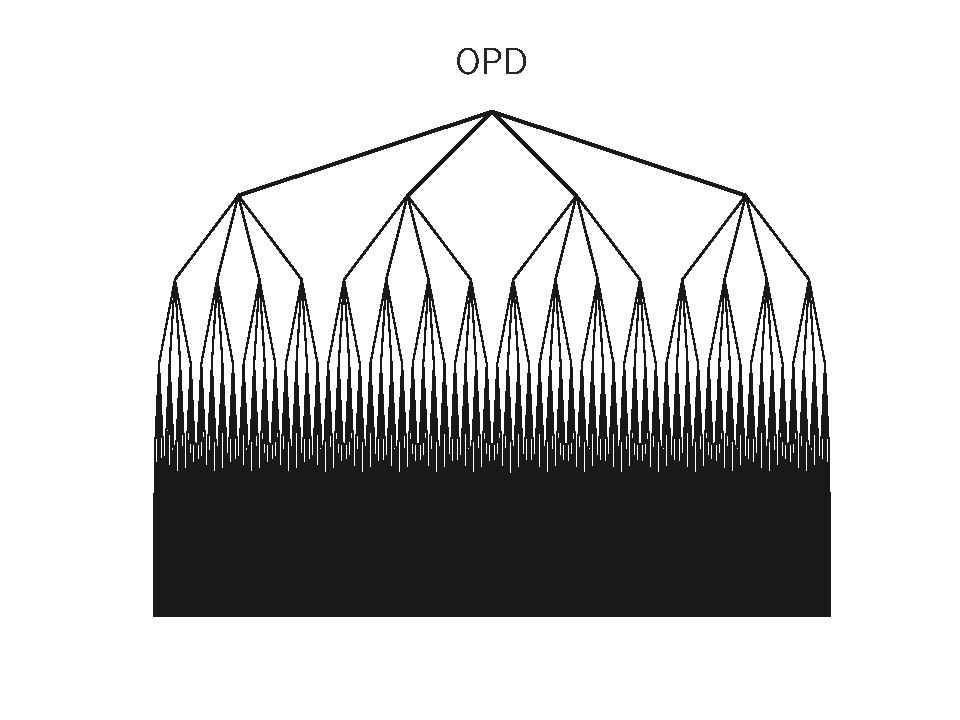
\includegraphics[trim={0 0.5cm 0 0.5cm}, clip, width=0.85\linewidth]{img/tree_OPD.pdf}
    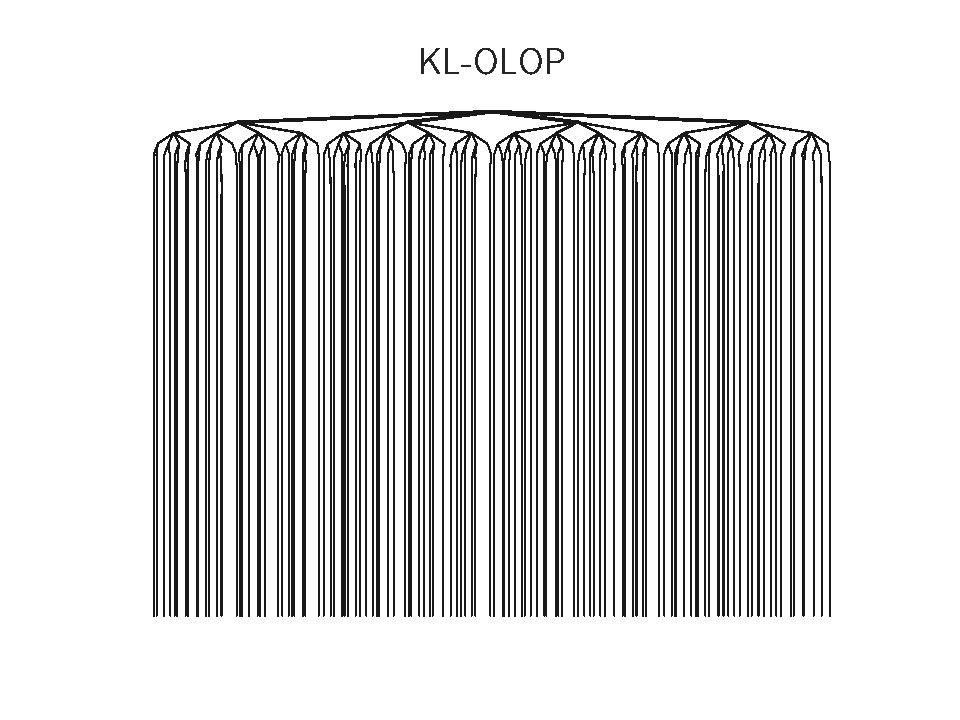
\includegraphics[trim={0 0.5cm 0 0.5cm}, clip, width=0.85\linewidth]{img/tree_KL-OLOP.pdf}
	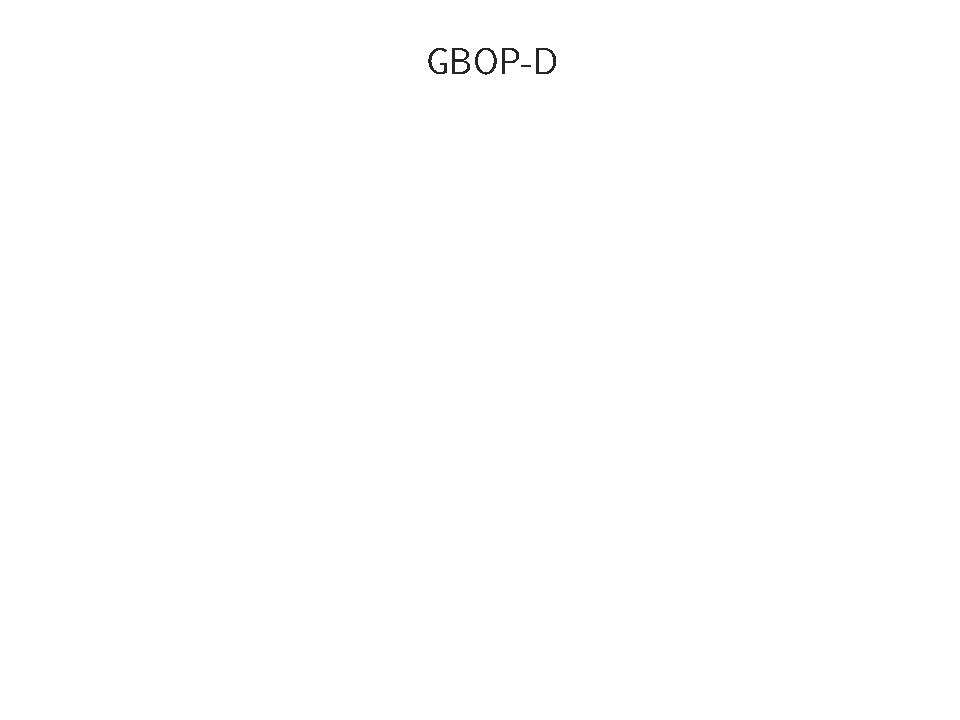
\includegraphics[trim={0 0.5cm 0 0.5cm}, clip, width=0.85\linewidth]{img/tree_GBOP-D.pdf}
	\caption{Trees expanded by \OPD, by \texttt{KL-OLOP}, and sequences of actions sampled by \GBOPD. The width of edges is proportional to the number of visits.}
	\label{fig:suppl-trees}
\end{figure}

%\end{comment}

\end{document}
